\documentclass[12pt,a4paper,openany]{report}
\usepackage[T1]{fontenc}
\usepackage{lmodern}
\usepackage[margin=1in]{geometry}
\usepackage{tabularx}
\usepackage{booktabs}
\usepackage{longtable}
\usepackage{titlesec}
\titlespacing*{\chapter}{0pt}{0pt}{18pt}
\titlespacing*{\section}{0pt}{8pt}{2pt}
\usepackage{tikz}
\usetikzlibrary{positioning,calc,arrows.meta}

\definecolor{apexfill}{HTML}{DCE6F1}
\definecolor{apexline}{HTML}{2F5496}
\definecolor{subfill}{HTML}{F2F2F2}
\definecolor{subline}{HTML}{666666}
\definecolor{cabfill}{HTML}{BDD7EE}
\definecolor{cabline}{HTML}{1F4E79}
\definecolor{mosfill}{HTML}{FCE4D6}
\definecolor{mosline}{HTML}{C55A11}
\definecolor{cmred}{HTML}{C00000}
\hyphenation{Chancellorship direction}

\tikzset{
  hroot/.style={draw=apexline, fill=apexfill, rounded corners=4pt,
                line width=0.8pt, text width=3.6cm, align=center,
                minimum height=1.25cm, font=\bfseries,
                execute at begin node={\hyphenpenalty=10000\relax}},
  hlvl/.style={draw=apexline!70, fill=apexfill!60, rounded corners=3pt,
               line width=0.7pt, text width=3.2cm, align=center,
               minimum height=1.1cm, font=\small,
               execute at begin node={\hyphenpenalty=10000\relax}},
  hsub/.style={draw=subline, fill=subfill, rounded corners=3pt,
               line width=0.6pt, text width=2.7cm, align=center,
               minimum height=1.0cm, font=\small,
               execute at begin node={\hyphenpenalty=10000\relax}},
  hleaf/.style={draw=subline, fill=subfill!75, rounded corners=3pt,
                line width=0.6pt, text width=2.7cm, align=center,
                minimum height=0.9cm, font=\footnotesize,
                execute at begin node={\hyphenpenalty=10000\relax}},
  cabbox/.style={draw=cabline, fill=cabfill, rounded corners=3pt,
                 line width=0.8pt, text width=3.4cm, align=center,
                 minimum height=1.1cm, font=\bfseries\small},
  mosbox/.style={draw=mosline, fill=mosfill, rounded corners=3pt,
                 line width=0.8pt, text width=3.4cm, align=center,
                 minimum height=1.1cm, font=\bfseries\small},
  minbox/.style={draw=subline, fill=subfill!70, rounded corners=2pt,
                 line width=0.5pt, text width=3.4cm, align=center,
                 minimum height=0.9cm, font=\scriptsize,
                 execute at begin node={\hyphenpenalty=10000\relax}},
  hlink/.style={draw=black!65, line width=0.7pt},
  fnbox/.style={draw=apexline!55, fill=apexfill!45, rounded corners=3pt,
                line width=0.6pt, text width=5.5cm, align=left,
                minimum height=2.6cm, font=\footnotesize, inner sep=6pt,
                execute at begin node={\hyphenpenalty=10000\relax}},
  elecbox/.style={draw=apexline!70, fill=apexfill!45, rounded corners=3pt,
                  line width=0.7pt, text width=10.8cm, align=center,
                  minimum height=1.45cm, font=\small,
                  execute at begin node={\hyphenpenalty=10000\relax}},
  secbox/.style={draw=apexline!55, fill=apexfill!30, rounded corners=3pt,
                 line width=0.6pt, text width=7.1cm, align=left,
                 minimum height=4.0cm, font=\scriptsize, inner sep=7pt,
                 anchor=north,
                 execute at begin node={\hyphenpenalty=10000\relax}}
}

\begin{document}

% ---------------------------------------------------------------- title page
\begin{titlepage}
  \centering
  \vspace*{4.5cm}
  {\Huge\bfseries Indian Union Administration\par}
  \vspace{0.6cm}
  {\Large The National Administrative Hierarchy\par}
  \vspace{0.35cm}
  {\large From the President of India to a Village Panchayat at Muri\par}
  \vfill
  {\small Office holders as of October 2026\par}
\end{titlepage}

% ---------------------------------------------------------------- apex page
\begin{center}
\resizebox{\textwidth}{!}{%
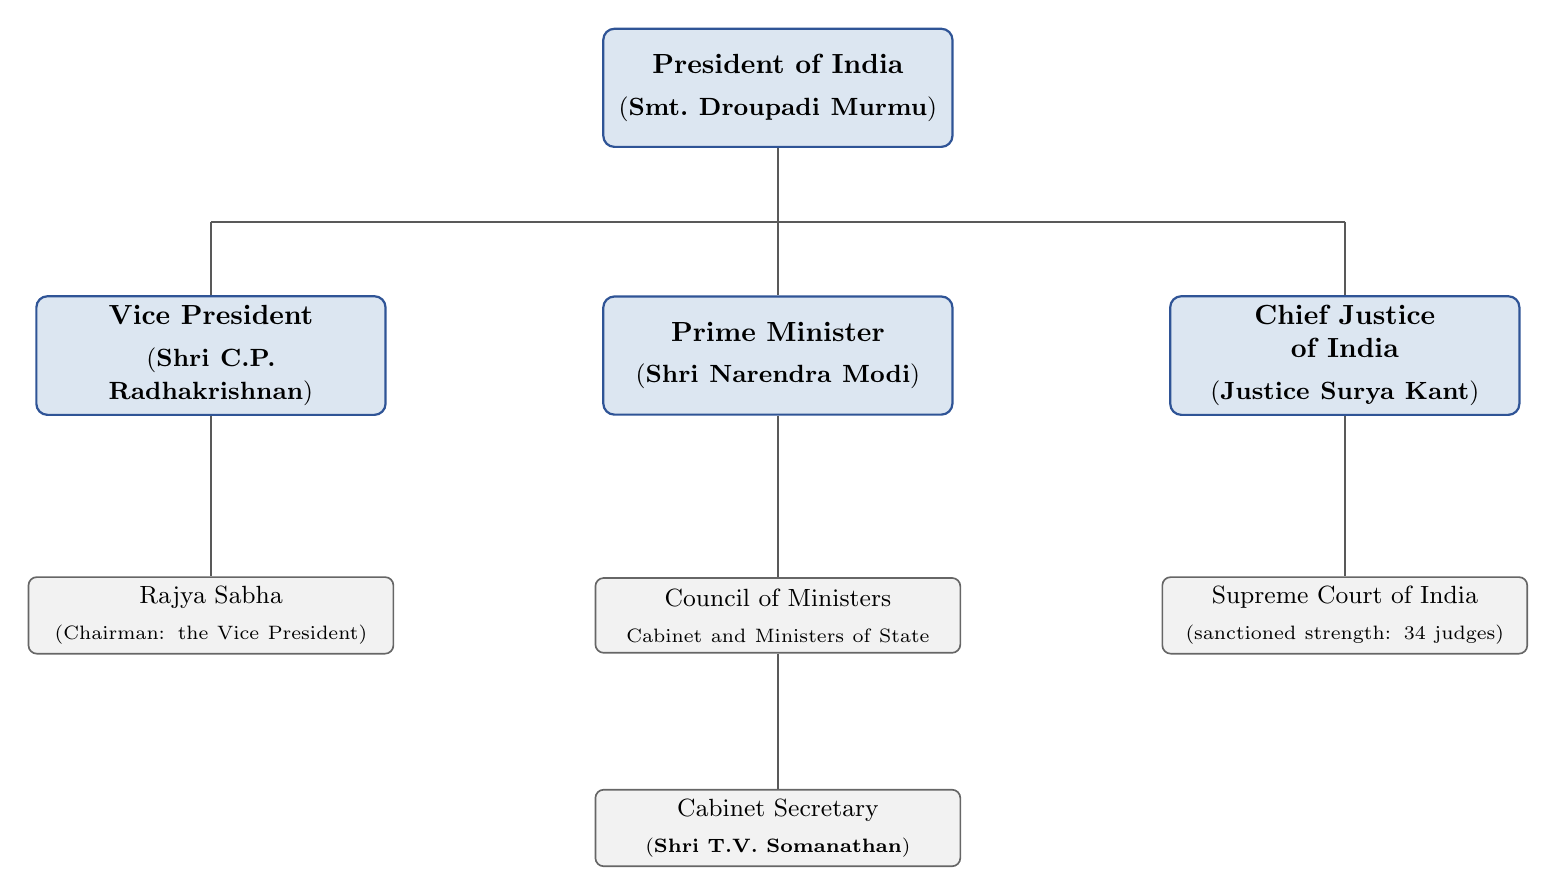
\begin{tikzpicture}[
  apex/.style={draw=apexline, fill=apexfill, rounded corners=4pt,
               line width=0.8pt, text width=4.2cm, align=center,
               minimum height=1.5cm, font=\bfseries,
               execute at begin node={\hyphenpenalty=10000\relax}},
  sub/.style={draw=subline, fill=subfill, rounded corners=3pt,
              line width=0.6pt, text width=4.4cm, align=center,
              minimum height=0.95cm, font=\small},
  link/.style={draw=black!65, line width=0.8pt}
]

% ---- apex level -----------------------------------------------------------
\node[apex] (pres) at (0,0)
  {President of India\\[3pt]{\normalfont\small (\textbf{Smt.\ Droupadi Murmu})}};

\node[apex] (vp) at (-7.2,-3.4)
  {Vice President\\[3pt]{\normalfont\small (\textbf{Shri C.P.\ Radhakrishnan})}};

\node[apex] (pm) at (0,-3.4)
  {Prime Minister\\[3pt]{\normalfont\small (\textbf{Shri Narendra Modi})}};

\node[apex] (cji) at (7.2,-3.4)
  {Chief Justice\\of India\\[3pt]{\normalfont\small (\textbf{Justice Surya Kant})}};

% ---- third level ----------------------------------------------------------
\node[sub] (rs) at (-7.2,-6.7)
  {Rajya Sabha\\[2pt]{\scriptsize (Chairman: the Vice President)}};

\node[sub] (com) at (0,-6.7)
  {Council of Ministers\\[2pt]{\scriptsize Cabinet and Ministers of State}};

\node[sub] (sc) at (7.2,-6.7)
  {Supreme Court of India\\[2pt]{\scriptsize (sanctioned strength: 34 judges)}};

\node[sub] (cs) at (0,-9.4)
  {Cabinet Secretary\\[2pt]{\scriptsize (\textbf{Shri T.V.\ Somanathan})}};

% ---- links ----------------------------------------------------------------
\draw[link] (pres.south) -- (0,-1.7);
\draw[link] (-7.2,-1.7) -- (7.2,-1.7);
\draw[link] (-7.2,-1.7) -- (vp.north);
\draw[link] (0,-1.7) -- (pm.north);
\draw[link] (7.2,-1.7) -- (cji.north);

\draw[link] (vp.south) -- (rs.north);
\draw[link] (cji.south) -- (sc.north);
\draw[link] (pm.south) -- (com.north);
\draw[link] (com.south) -- (cs.north);

\end{tikzpicture}%
}
\end{center}

\section*{How These Apex Offices Inter-relate}

\noindent{\scriptsize
\renewcommand{\arraystretch}{1.2}%
\begin{tabularx}{\textwidth}{@{}>{\raggedright\arraybackslash}p{3.3cm} X >{\raggedright\arraybackslash}p{3.2cm}@{}}
\toprule
\textbf{Pair} & \textbf{Nature of relation} & \textbf{Basis} \\
\midrule
President $\leftrightarrow$ Vice President &
The Vice President is ex officio Chairman of the Rajya Sabha; on a vacancy in the office of President he acts as President, and if that vacancy is prolonged he discharges the functions until a new President is elected. &
Arts.\ 63--65 \\
\addlinespace[4pt]
President $\leftrightarrow$ Prime Minister &
The President appoints the Prime Minister and, on the PM's advice, the other Ministers. The President exercises the executive power of the Union on the aid and advice of the Council of Ministers headed by the Prime Minister. &
Arts.\ 74, 75 \\
\addlinespace[4pt]
President $\leftrightarrow$ Council of Ministers &
The Council is collectively responsible to the Lok Sabha. The President summons and prorogues Parliament, dissolves the Lok Sabha, and assents to, withholds assent from, or returns Bills. &
Arts.\ 74, 75(3), 85, 111 \\
\addlinespace[4pt]
President $\leftrightarrow$ Chief Justice of India &
The President appoints the Chief Justice and the other judges of the Supreme Court and the High Courts; the Chief Justice is consulted on appointments and is the head of the judiciary. &
Arts.\ 124, 217 \\
\addlinespace[4pt]
President $\leftrightarrow$ Governors &
Governors are appointed by the President and hold office during his pleasure; the Governor's report is the usual route to President's Rule in a State. &
Arts.\ 155, 356 \\
\addlinespace[4pt]
Prime Minister $\leftrightarrow$ Cabinet Secretary &
The PM chairs the Cabinet; the Cabinet Secretary is Secretary to the Cabinet and the administrative head of the civil service, and answers to the PM and the Cabinet. &
Executive practice \\
\bottomrule
\end{tabularx}}

\vspace{2pt}
\noindent\textbf{Flow of authority:} President (appoints, assents) $\leftrightarrow$ Prime Minister (directs) $\rightarrow$ Council of Ministers $\rightarrow$ Cabinet Secretary (implements) $\rightarrow$ Secretaries of Ministries $\rightarrow$ field administration in the States and districts.

\noindent\textbf{Accountability:} the Council of Ministers to the Lok Sabha; the Cabinet Secretary to the PM and Cabinet; the President to the Constitution and, in impeachment, to Parliament.

% ======================================================= under the President
\newpage
\section*{Hierarchies under the President}

\begin{center}
\resizebox{\textwidth}{!}{%
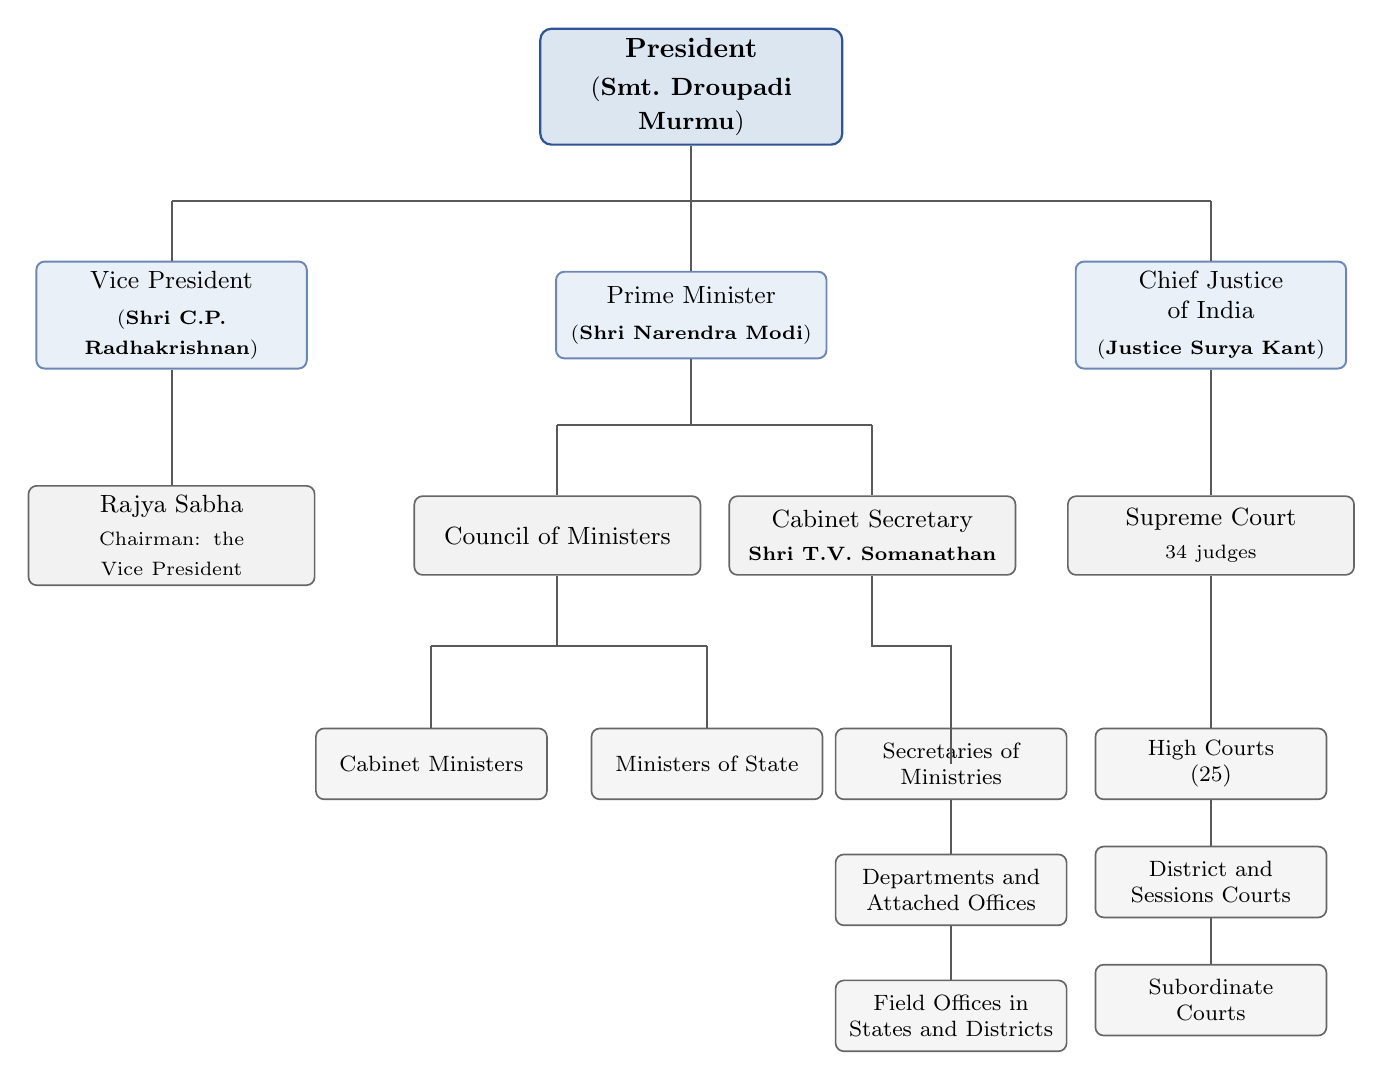
\begin{tikzpicture}
  \node[hroot] (pres) at (0,0)
    {President\\[2pt]{\normalfont\small (\textbf{Smt.\ Droupadi Murmu})}};

  \node[hlvl] (vp) at (-6.6,-2.9)
    {Vice President\\[2pt]{\normalfont\scriptsize (\textbf{Shri C.P.\ Radhakrishnan})}};
  \node[hlvl] (pm) at (0,-2.9)
    {Prime Minister\\[2pt]{\normalfont\scriptsize (\textbf{Shri Narendra Modi})}};
  \node[hlvl] (cji) at (6.6,-2.9)
    {Chief Justice\\of India\\[2pt]{\normalfont\scriptsize (\textbf{Justice Surya Kant})}};

  \node[hsub, text width=3.4cm] (rs) at (-6.6,-5.7)
    {Rajya Sabha\\[1pt]{\scriptsize Chairman: the Vice President}};
  \node[hsub, text width=3.4cm] (com) at (-1.7,-5.7) {Council of Ministers};
  \node[hsub, text width=3.4cm] (csec) at (2.3,-5.7)
    {Cabinet Secretary\\[1pt]{\scriptsize \textbf{Shri T.V.\ Somanathan}}};
  \node[hsub, text width=3.4cm] (sc) at (6.6,-5.7) {Supreme Court\\[1pt]{\scriptsize 34 judges}};

  \node[hleaf] (cab) at (-3.3,-8.6) {Cabinet Ministers};
  \node[hleaf] (mos) at (0.2,-8.6) {Ministers of State};
  \node[hleaf] (sec) at (3.3,-8.6) {Secretaries of\\Ministries};

  \node[hleaf] (hc) at (6.6,-8.6) {High Courts\\(25)};
  \node[hleaf] (dc) at (6.6,-10.1) {District and\\Sessions Courts};
  \node[hleaf] (sub) at (6.6,-11.6) {Subordinate\\Courts};

  \node[hleaf] (dep) at (3.3,-10.2) {Departments and\\Attached Offices};
  \node[hleaf] (field) at (3.3,-11.8) {Field Offices in\\States and Districts};

  \draw[hlink] (pres.south) -- (0,-1.45);
  \draw[hlink] (-6.6,-1.45) -- (6.6,-1.45);
  \draw[hlink] (-6.6,-1.45) -- (vp.north);
  \draw[hlink] (0,-1.45) -- (pm.north);
  \draw[hlink] (6.6,-1.45) -- (cji.north);

  \draw[hlink] (vp.south) -- (rs.north);
  \draw[hlink] (cji.south) -- (sc.north);

  \draw[hlink] (pm.south) -- (0,-4.3);
  \draw[hlink] (-1.7,-4.3) -- (2.3,-4.3);
  \draw[hlink] (-1.7,-4.3) -- (com.north);
  \draw[hlink] (2.3,-4.3) -- (csec.north);

  \draw[hlink] (com.south) -- (-1.7,-7.1);
  \draw[hlink] (-3.3,-7.1) -- (0.2,-7.1);
  \draw[hlink] (-3.3,-7.1) -- (cab.north);
  \draw[hlink] (0.2,-7.1) -- (mos.north);

  \draw[hlink] (csec.south) -- (2.3,-7.1) -- (3.3,-7.1) -- (3.3,-8.6);
  \draw[hlink] (3.3,-7.1) -- (sec.north);
  \draw[hlink] (sec.south) -- (sec.south |- dep.north);
  \draw[hlink] (dep.south) -- (field.north);

  \draw[hlink] (sc.south) -- (hc.north);
  \draw[hlink] (hc.south) -- (dc.north);
  \draw[hlink] (dc.south) -- (sub.north);
\end{tikzpicture}%
}
\end{center}

\section*{Nature of the Blue Boxes}

\noindent{\scriptsize
\renewcommand{\arraystretch}{1.12}%
\begin{tabularx}{\textwidth}{@{}>{\raggedright\arraybackslash}p{2.9cm} >{\raggedright\arraybackslash}p{6.3cm} >{\raggedright\arraybackslash}X@{}}
\toprule
\textbf{Box} & \textbf{Nature of the office} & \textbf{Core mandate} \\
\midrule
President & Constitutional head of the Union; Supreme Commander of the Armed Forces; not a member of either House. & Appointments, assent to legislation, emergency powers, and the care that the Constitution is faithfully executed. \\
\addlinespace[2pt]
Vice President & Second constitutional office; ex officio Chairman of the Rajya Sabha. & Presides over the Rajya Sabha and acts as President on a vacancy. \\
\addlinespace[2pt]
Prime Minister & Head of the Government; leader of the majority in the Lok Sabha. & Formation of the Council, allocation of portfolios, policy direction and answerability to the House. \\
\addlinespace[2pt]
Chief Justice of India & Head of the judiciary; senior-most judge of the Supreme Court. & Administration of the Supreme Court, consultation on judicial appointments and the constitutional jurisdiction of the Court. \\
\addlinespace[2pt]
Cabinet Secretary & Non-constitutional administrative head; senior-most IAS officer; Secretary to the Cabinet. & Coordination among Secretaries, the Cabinet Secretariat, and monitoring of the Government's priority programmes. \\
\bottomrule
\end{tabularx}}

% ======================================================= cabinet ministers
\newpage
\section*{The Union Council of Ministers: Cabinet Ministers}

\noindent{\footnotesize The Council of Ministers is appointed by the President on the advice of the Prime Minister. It consists of Cabinet Ministers, Ministers of State with independent charge, and Ministers of State attached to Cabinet Ministers. Portfolios below are as of October 2026.}

\vspace{4pt}
\noindent{\footnotesize
\renewcommand{\arraystretch}{1.16}%
\begin{longtable}{@{}>{\raggedright\arraybackslash}p{8.3cm} >{\raggedright\arraybackslash}p{7.1cm}@{}}
\toprule
\textbf{Portfolio} & \textbf{Cabinet Minister} \\
\midrule
\endfirsthead
\toprule
\textbf{Portfolio} & \textbf{Cabinet Minister} \\
\midrule
\endhead
Prime Minister; Personnel, Public Grievances and Pensions; Department of Atomic Energy; Department of Space; all portfolios not allotted to any other Minister & \textbf{Shri Narendra Modi} \\
\addlinespace[2pt]
Defence & \textbf{Shri Rajnath Singh} \\
\addlinespace[2pt]
Home Affairs; Cooperation & \textbf{Shri Amit Shah} \\
\addlinespace[2pt]
Road Transport and Highways & \textbf{Shri Nitin Gadkari} \\
\addlinespace[2pt]
Health and Family Welfare; Chemicals and Fertilizers & \textbf{Shri Jagat Prakash Nadda} \\
\addlinespace[2pt]
Agriculture and Farmers Welfare; Rural Development & \textbf{Shri Shivraj Singh Chouhan} \\
\addlinespace[2pt]
Finance; Corporate Affairs & \textbf{Smt.\ Nirmala Sitharaman} \\
\addlinespace[2pt]
External Affairs & \textbf{Dr.\ Subrahmanyam Jaishankar} \\
\addlinespace[2pt]
Housing and Urban Affairs; Power & \textbf{Shri Manohar Lal Khattar} \\
\addlinespace[2pt]
Heavy Industries; Steel & \textbf{Shri H.D.\ Kumaraswamy} \\
\addlinespace[2pt]
Commerce and Industry & \textbf{Shri Piyush Goyal} \\
\addlinespace[2pt]
Education & \textbf{Shri Dharmendra Pradhan} \\
\addlinespace[2pt]
Micro, Small and Medium Enterprises & \textbf{Shri Jitan Ram Manjhi} \\
\addlinespace[2pt]
Panchayati Raj; Fisheries, Animal Husbandry and Dairying & \textbf{Shri Rajiv Ranjan Singh (Lalan Singh)} \\
\addlinespace[2pt]
Ports, Shipping and Waterways & \textbf{Shri Sarbananda Sonowal} \\
\addlinespace[2pt]
Social Justice and Empowerment & \textbf{Dr.\ Virendra Kumar} \\
\addlinespace[2pt]
Civil Aviation & \textbf{Shri Kinjarapu Rammohan Naidu} \\
\addlinespace[2pt]
Consumer Affairs, Food and Public Distribution; New and Renewable Energy & \textbf{Shri Pralhad Joshi} \\
\addlinespace[2pt]
Tribal Affairs & \textbf{Shri Jual Oram} \\
\addlinespace[2pt]
Textiles & \textbf{Shri Giriraj Singh} \\
\addlinespace[2pt]
Railways; Information and Broadcasting; Electronics and Information Technology & \textbf{Shri Ashwini Vaishnaw} \\
\addlinespace[2pt]
Communications; Development of North Eastern Region & \textbf{Shri Jyotiraditya Scindia} \\
\addlinespace[2pt]
Environment, Forest and Climate Change & \textbf{Shri Bhupender Yadav} \\
\addlinespace[2pt]
Labour and Employment; Youth Affairs and Sports & \textbf{Dr.\ Mansukh Mandaviya} \\
\addlinespace[2pt]
Coal; Mines & \textbf{Shri G.\ Kishan Reddy} \\
\addlinespace[2pt]
Food Processing Industries & \textbf{Shri Chirag Paswan} \\
\addlinespace[2pt]
Jal Shakti & \textbf{Shri C.R.\ Patil} \\
\addlinespace[2pt]
Petroleum and Natural Gas & \textbf{Shri Hardeep Singh Puri} \\
\addlinespace[2pt]
Parliamentary Affairs; Minority Affairs & \textbf{Shri Kiren Rijiju} \\
\addlinespace[2pt]
Tourism; Culture & \textbf{Shri Gajendra Singh Shekhawat} \\
\addlinespace[2pt]
Women and Child Development & \textbf{Smt.\ Annapurna Devi} \\
\bottomrule
\end{longtable}}

% ======================================================= ministers of state
\newpage
\section*{The Union Council of Ministers: Ministers of State}

\noindent{\footnotesize Ministers of State either hold independent charge of one or more departments, or assist a Cabinet Minister in the subjects allotted to them.}

\vspace{4pt}
\noindent{\footnotesize\textbf{Ministers of State with Independent Charge}}

\vspace{2pt}
\noindent{\footnotesize
\renewcommand{\arraystretch}{1.16}%
\begin{longtable}{@{}>{\raggedright\arraybackslash}p{8.3cm} >{\raggedright\arraybackslash}p{7.1cm}@{}}
\toprule
\textbf{Portfolio} & \textbf{Minister of State (Independent Charge)} \\
\midrule
\endfirsthead
\toprule
\textbf{Portfolio} & \textbf{Minister of State (Independent Charge)} \\
\midrule
\endhead
Statistics and Programme Implementation; Planning & \textbf{Shri Rao Inderjit Singh} \\
\addlinespace[2pt]
Science and Technology; Earth Sciences; Prime Minister's Office; Personnel, Public Grievances and Pensions; Atomic Energy; Space & \textbf{Dr.\ Jitendra Singh} \\
\addlinespace[2pt]
Law and Justice & \textbf{Shri Arjun Ram Meghwal} \\
\addlinespace[2pt]
Skill Development and Entrepreneurship & \textbf{Shri Jayant Chaudhary} \\
\addlinespace[2pt]
Ayush & \textbf{Shri Prataprao Jadhav} \\
\bottomrule
\end{longtable}}

\vspace{6pt}
\noindent{\footnotesize\textbf{Ministers of State attached to Cabinet Ministers}}

\vspace{2pt}
\noindent{\footnotesize
\renewcommand{\arraystretch}{1.16}%
\begin{longtable}{@{}>{\raggedright\arraybackslash}p{8.3cm} >{\raggedright\arraybackslash}p{7.1cm}@{}}
\toprule
\textbf{Portfolio} & \textbf{Minister of State} \\
\midrule
\endfirsthead
\toprule
\textbf{Portfolio} & \textbf{Minister of State} \\
\midrule
\endhead
Commerce and Industry; Electronics and Information Technology & \textbf{Shri Jitin Prasada} \\
\addlinespace[2pt]
Power; New and Renewable Energy & \textbf{Shri Shripad Naik} \\
\addlinespace[2pt]
Finance & \textbf{Shri Pankaj Chaudhary} \\
\addlinespace[2pt]
Cooperation & \textbf{Shri Krishan Pal Gurjar} \\
\addlinespace[2pt]
Social Justice and Empowerment & \textbf{Shri Ramdas Athawale} \\
\addlinespace[2pt]
Agriculture and Farmers Welfare & \textbf{Shri Ram Nath Thakur} \\
\addlinespace[2pt]
Home Affairs & \textbf{Shri Nityanand Rai} \\
\addlinespace[2pt]
Health and Family Welfare; Chemicals and Fertilizers & \textbf{Smt.\ Anupriya Patel} \\
\addlinespace[2pt]
Jal Shakti; Railways & \textbf{Shri V.\ Somanna} \\
\addlinespace[2pt]
Rural Development; Communications & \textbf{Dr.\ Chandra Sekhar Pemmasani} \\
\addlinespace[2pt]
Fisheries, Animal Husbandry and Dairying; Panchayati Raj & \textbf{Prof.\ S.P.\ Singh Baghel} \\
\addlinespace[2pt]
Micro, Small and Medium Enterprises; Labour and Employment & \textbf{Smt.\ Shobha Karandlaje} \\
\addlinespace[2pt]
Environment, Forest and Climate Change; External Affairs & \textbf{Shri Kirti Vardhan Singh} \\
\addlinespace[2pt]
Social Justice and Empowerment; Cooperation & \textbf{Shri B.L.\ Verma} \\
\addlinespace[2pt]
Ports, Shipping and Waterways & \textbf{Shri Shantanu Thakur} \\
\addlinespace[2pt]
Petroleum and Natural Gas; Tourism & \textbf{Shri Suresh Gopi} \\
\addlinespace[2pt]
Information and Broadcasting; Parliamentary Affairs & \textbf{Dr.\ L.\ Murugan} \\
\addlinespace[2pt]
Road Transport and Highways; Micro, Small and Medium Enterprises & \textbf{Shri Ajay Tamta} \\
\addlinespace[2pt]
Home Affairs & \textbf{Shri Bandi Sanjay Kumar} \\
\addlinespace[2pt]
Rural Development & \textbf{Shri Kamlesh Paswan} \\
\addlinespace[2pt]
Agriculture and Farmers Welfare & \textbf{Shri Bhagirath Choudhary} \\
\addlinespace[2pt]
Coal; Mines & \textbf{Shri Satish Chandra Dubey} \\
\addlinespace[2pt]
Defence & \textbf{Shri Sanjay Seth} \\
\addlinespace[2pt]
Railways; Food Processing Industries & \textbf{Shri Ravneet Singh Bittu} \\
\addlinespace[2pt]
Tribal Affairs & \textbf{Shri Durgadas Uikey} \\
\addlinespace[2pt]
Youth Affairs and Sports; Women and Child Development & \textbf{Smt.\ Raksha Nikhil Khadse} \\
\addlinespace[2pt]
Education; Development of North Eastern Region & \textbf{Dr.\ Sukanta Majumdar} \\
\addlinespace[2pt]
Women and Child Development & \textbf{Smt.\ Savitri Thakur} \\
\addlinespace[2pt]
Housing and Urban Affairs & \textbf{Shri Tokhan Sahu} \\
\addlinespace[2pt]
Jal Shakti & \textbf{Shri Raj Bhushan Choudhary} \\
\addlinespace[2pt]
Heavy Industries; Steel & \textbf{Shri Bhupathiraju Srinivasa Varma} \\
\addlinespace[2pt]
Corporate Affairs; Road Transport and Highways & \textbf{Shri Harsh Malhotra} \\
\addlinespace[2pt]
Consumer Affairs, Food and Public Distribution & \textbf{Smt.\ Nimuben Jayantibhai Bambhaniya} \\
\addlinespace[2pt]
Cooperation; Civil Aviation & \textbf{Shri Murlidhar Mohol} \\
\addlinespace[2pt]
Minority Affairs; Fisheries, Animal Husbandry and Dairying & \textbf{Shri George Kurian} \\
\addlinespace[2pt]
External Affairs; Textiles & \textbf{Shri Pabitra Margherita} \\
\bottomrule
\end{longtable}}

\noindent{\scriptsize As per the allocation notified by the President on the advice of the Prime Minister; subject to reshuffle.}

% ======================================================= cabinet vs mos
\section*{Cabinet Minister vs Minister of State}

\noindent{\footnotesize
\renewcommand{\arraystretch}{1.24}%
\begin{tabularx}{\textwidth}{@{}>{\raggedright\arraybackslash}p{2.8cm} >{\raggedright\arraybackslash}X >{\raggedright\arraybackslash}X@{}}
\toprule
 & \textbf{Cabinet Minister} & \textbf{Minister of State} \\
\midrule
Rank & Senior minister of Cabinet rank; heads a ministry and sits in the Cabinet. & Junior minister; assists a Cabinet Minister, or holds independent charge of a department. \\
\addlinespace[3pt]
Cabinet & Attends Cabinet meetings and shares in collective decisions. & Attends only if specially invited. \\
\addlinespace[3pt]
Work & Sets the ministry's policy, supervises its departments and answers for the whole ministry in the House. & Runs the allotted subjects, assists the Cabinet Minister and represents the ministry in the House. \\
\addlinespace[3pt]
Accountability & Collective responsibility (Art.~75(3)); answerable for the entire ministry. & Same collective responsibility; answerable for the allotted work. \\
\bottomrule
\end{tabularx}}

\vspace{4pt}
\noindent{\footnotesize All ministers are appointed by the President on the advice of the Prime Minister, and must be, or become within six months, members of either House of Parliament.}

\vspace{6pt}
\noindent{\footnotesize\textbf{How they function.} The Cabinet Minister decides; the Minister of State executes the allotted part and carries the ministry's case in the House. Both work through the same Secretaries, and the Cabinet Minister remains answerable for the ministry as a whole. A Minister of State with independent charge is treated as the head of the department for its day-to-day administration but does not sit in the Cabinet.}

% ======================================================= constitutional bodies
\newpage
\section*{Constitutional and Statutory Authorities}

\noindent{\scriptsize
\renewcommand{\arraystretch}{1.1}%
\begin{longtable}{@{}>{\raggedright\arraybackslash}p{3.5cm} >{\raggedright\arraybackslash}p{4.6cm} >{\raggedright\arraybackslash}p{2.2cm} >{\raggedright\arraybackslash}p{4.3cm}@{}}
\toprule
\textbf{Body} & \textbf{Head (October 2026)} & \textbf{Basis} & \textbf{Core function} \\
\midrule
\endfirsthead
\toprule
\textbf{Body} & \textbf{Head (October 2026)} & \textbf{Basis} & \textbf{Core function} \\
\midrule
\endhead
Election Commission of India & Chief Election Commissioner \textbf{Shri Gyanesh Kumar}; Election Commissioners \textbf{Shri Sukhbir Singh Sandhu} and \textbf{Shri Vivek Joshi} & Art.\ 324 & Superintendence, direction and control of elections to Parliament, State legislatures, the offices of President and Vice President. \\
\addlinespace[2pt]
Comptroller and Auditor General & \textbf{Shri K.\ Sanjay Murthy} & Arts.\ 148--151 & Audit of all Union and State accounts; reports laid before Parliament. \\
\addlinespace[2pt]
Union Public Service Commission & Chairperson \textbf{Smt.\ Preeti Sudan} & Arts.\ 315--323 & Recruitment to the All India Services and Central Services; advice on service matters. \\
\addlinespace[2pt]
Finance Commission & Chairman \textbf{Dr.\ Arvind Panagariya} & Art.\ 280 & Recommends the distribution of net proceeds of taxes between the Union and the States and grants-in-aid. \\
\addlinespace[2pt]
Attorney General of India & \textbf{Shri R.\ Venkataramani} & Art.\ 76 & Chief law officer; advises the Government on legal questions and appears for the Union in the courts. \\
\addlinespace[2pt]
Solicitor General of India & \textbf{Shri Tushar Mehta} & Statutory & Second law officer; assists the Attorney General and represents the Union in important litigation. \\
\addlinespace[2pt]
NITI Aayog & Chairperson \textbf{Shri Narendra Modi}; Vice-Chairman \textbf{Shri Suman Bery}; CEO \textbf{Shri B.V.R.\ Subrahmanyam} & Executive resolution, 2015 & Policy think tank; cooperative and competitive federalism; monitoring of national priorities. \\
\addlinespace[2pt]
Reserve Bank of India & Governor \textbf{Shri Sanjay Malhotra} & RBI Act, 1934 & Monetary policy, currency, regulation of the banking and payment systems. \\
\addlinespace[2pt]
National Human Rights Commission & Chairperson \textbf{Justice V.\ Ramasubramanian} & Protection of Human Rights Act, 1993 & Inquiry into complaints of violation of human rights; review of safeguards. \\
\addlinespace[2pt]
Lokpal & Chairperson \textbf{Justice A.M.\ Khanwilkar} & Lokpal and Lokayuktas Act, 2013 & Inquiry into allegations of corruption against public functionaries. \\
\addlinespace[2pt]
Central Vigilance Commission & Central Vigilance Commissioner \textbf{Shri Praveen Kumar Srivastava} & CVC Act, 2003 & Vigilance oversight over public sector organisations. \\
\addlinespace[2pt]
Central Information Commission & Chief Information Commissioner \textbf{Shri Heeralal Samariya} & Right to Information Act, 2005 & Second appeal under the RTI Act; transparency oversight. \\
\addlinespace[2pt]
National Commission for Women & Chairperson \textbf{Smt.\ Vijaya Kishore Rahatkar} & NCW Act, 1990 & Review of laws and safeguards affecting women; complaints and policy advice. \\
\bottomrule
\end{longtable}}

\vspace{3pt}
\noindent{\scriptsize Names are as per the latest central records available in October 2026. Constitutional bodies are created by the Constitution; statutory bodies by an Act of Parliament.}

% ======================================================= judiciary
\newpage
\section*{The Judiciary: From the Supreme Court to the District Court}

\begin{center}
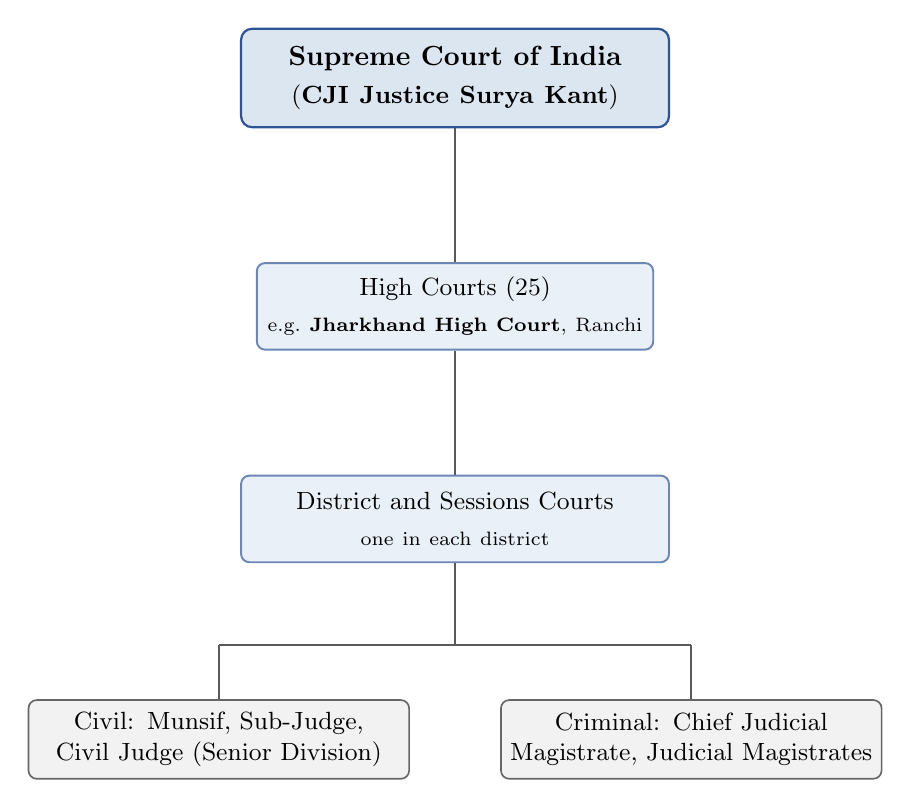
\begin{tikzpicture}
  \node[hroot, text width=5.2cm] (sc) at (0,0)
    {Supreme Court of India\\[2pt]{\normalfont\small (\textbf{CJI Justice Surya Kant})}};

  \node[hlvl, text width=4.8cm] (hc) at (0,-2.9)
    {High Courts (25)\\[2pt]{\normalfont\scriptsize e.g.\ \textbf{Jharkhand High Court}, Ranchi}};

  \node[hlvl, text width=5.2cm] (dc) at (0,-5.6)
    {District and Sessions Courts\\[2pt]{\normalfont\scriptsize one in each district}};

  \node[hsub, text width=4.6cm] (sub) at (-3.0,-8.4)
    {Civil: Munsif, Sub-Judge,\\Civil Judge (Senior Division)};
  \node[hsub, text width=4.6cm] (cri) at (3.0,-8.4)
    {Criminal: Chief Judicial\\Magistrate, Judicial Magistrates};

  \draw[hlink] (sc.south) -- (hc.north);
  \draw[hlink] (hc.south) -- (dc.north);
  \draw[hlink] (dc.south) -- (0,-7.2);
  \draw[hlink] (-3.0,-7.2) -- (3.0,-7.2);
  \draw[hlink] (-3.0,-7.2) -- (sub.north);
  \draw[hlink] (3.0,-7.2) -- (cri.north);
\end{tikzpicture}
\end{center}

\vspace{2pt}
\noindent{\footnotesize
\renewcommand{\arraystretch}{1.18}%
\begin{tabularx}{\textwidth}{@{}>{\raggedright\arraybackslash}p{5.0cm} >{\raggedright\arraybackslash}p{5.4cm} X@{}}
\toprule
\textbf{Court} & \textbf{Head} & \textbf{Seat and notes} \\
\midrule
Supreme Court of India & Chief Justice of India \textbf{Justice Surya Kant} & New Delhi; sanctioned strength 34; apex appellate and constitutional court. \\
\addlinespace[2pt]
Jharkhand High Court & Chief Justice \textbf{Justice Mahesh Sharadchandra Sonak} & Ranchi; highest court for Jharkhand; appeals from all district and subordinate courts in the State. \\
\addlinespace[2pt]
District and Sessions Court, Ranchi & District and Sessions Judge & Ranchi; tries serious civil and criminal cases in the district. \\
\addlinespace[2pt]
Subordinate courts & Chief Judicial Magistrate and Civil Judges & Across the district; the first tier for most disputes and prosecutions. \\
\bottomrule
\end{tabularx}}

\vspace{6pt}
\noindent{\footnotesize\textbf{The High Courts of India (25).}}

\vspace{2pt}
\noindent{\scriptsize
\renewcommand{\arraystretch}{1.08}%
\begin{tabularx}{\textwidth}{@{}>{\raggedright\arraybackslash}p{7.2cm} >{\raggedright\arraybackslash}p{4.4cm} X@{}}
\toprule
\textbf{High Court} & \textbf{Seat} & \textbf{Jurisdiction} \\
\midrule
\textbf{Allahabad High Court} & Prayagraj & Uttar Pradesh \\
\textbf{Andhra Pradesh High Court} & Amaravati & Andhra Pradesh \\
\textbf{Bombay High Court} & Mumbai & Maharashtra, Goa, Dadra and Nagar Haveli and Daman and Diu \\
\textbf{Calcutta High Court} & Kolkata & West Bengal, Andaman and Nicobar Islands \\
\textbf{Chhattisgarh High Court} & Bilaspur & Chhattisgarh \\
\textbf{Delhi High Court} & New Delhi & National Capital Territory of Delhi \\
\textbf{Gauhati High Court} & Guwahati & Assam, Nagaland, Mizoram, Arunachal Pradesh \\
\textbf{Gujarat High Court} & Ahmedabad & Gujarat \\
\textbf{Himachal Pradesh High Court} & Shimla & Himachal Pradesh \\
\textbf{Jammu and Kashmir and Ladakh High Court} & Srinagar / Jammu & Jammu and Kashmir, Ladakh \\
\textbf{Jharkhand High Court} & Ranchi & Jharkhand \\
\textbf{Karnataka High Court} & Bengaluru & Karnataka \\
\textbf{Kerala High Court} & Ernakulam & Kerala, Lakshadweep \\
\textbf{Madhya Pradesh High Court} & Jabalpur & Madhya Pradesh \\
\textbf{Madras High Court} & Chennai & Tamil Nadu, Puducherry \\
\textbf{Manipur High Court} & Imphal & Manipur \\
\textbf{Meghalaya High Court} & Shillong & Meghalaya \\
\textbf{Orissa High Court} & Cuttack & Odisha \\
\textbf{Patna High Court} & Patna & Bihar \\
\textbf{Punjab and Haryana High Court} & Chandigarh & Punjab, Haryana, Chandigarh \\
\textbf{Rajasthan High Court} & Jodhpur & Rajasthan \\
\textbf{Sikkim High Court} & Gangtok & Sikkim \\
\textbf{Telangana High Court} & Hyderabad & Telangana \\
\textbf{Tripura High Court} & Agartala & Tripura \\
\textbf{Uttarakhand High Court} & Nainital & Uttarakhand \\
\bottomrule
\end{tabularx}}

\vspace{2pt}
\noindent{\footnotesize The Supreme Court is the final court of appeal and the guardian of the Constitution; the High Courts supervise all courts within their territorial jurisdiction; the district and subordinate courts form the base of the pyramid.}

% ======================================================= parliament
\newpage
\section*{Parliament of India}

\begin{center}
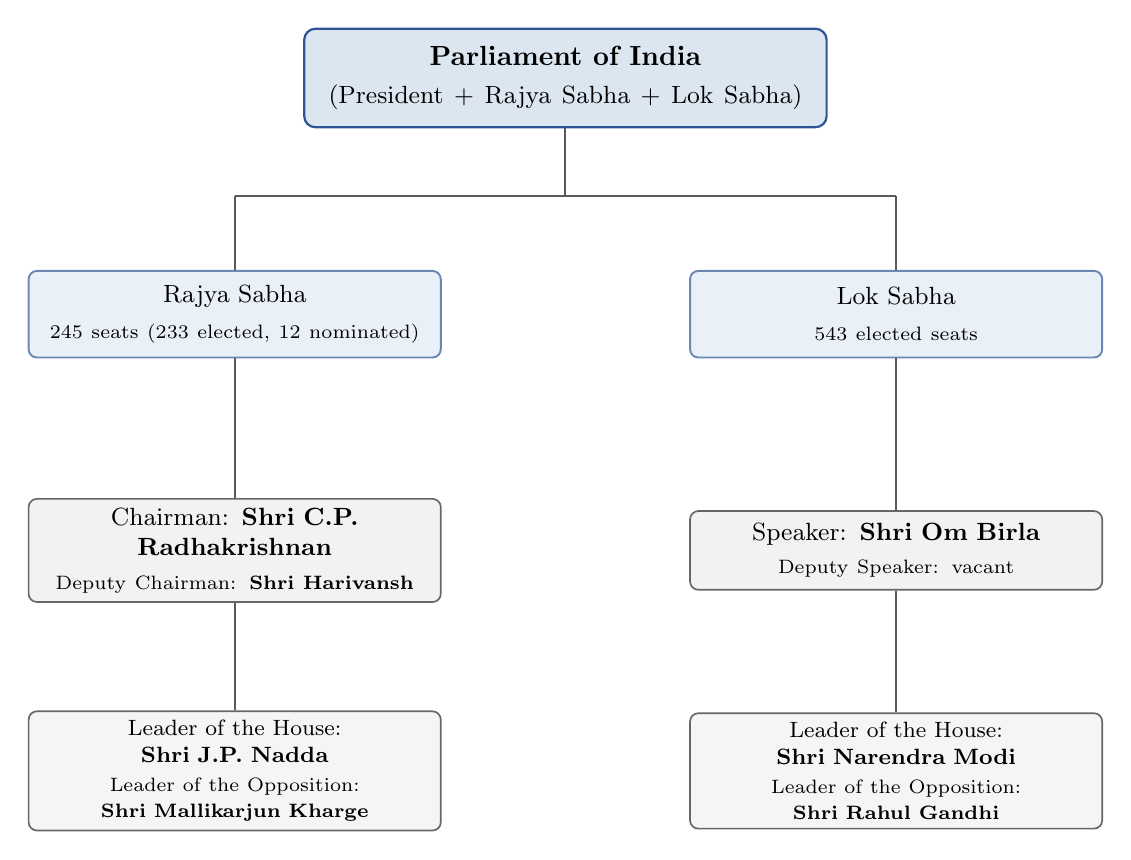
\begin{tikzpicture}
  \node[hroot, text width=6.4cm] (parl) at (0,0)
    {Parliament of India\\[2pt]{\normalfont\small (President + Rajya Sabha + Lok Sabha)}};

  \node[hlvl, text width=5.0cm] (rs) at (-4.2,-3.0)
    {Rajya Sabha\\[2pt]{\normalfont\scriptsize 245 seats (233 elected, 12 nominated)}};
  \node[hlvl, text width=5.0cm] (ls) at (4.2,-3.0)
    {Lok Sabha\\[2pt]{\normalfont\scriptsize 543 elected seats}};

  \node[hsub, text width=5.0cm] (rso) at (-4.2,-6.0)
    {Chairman: \textbf{Shri C.P.\ Radhakrishnan}\\[1pt]
     {\scriptsize Deputy Chairman: \textbf{Shri Harivansh}}};
  \node[hsub, text width=5.0cm] (lso) at (4.2,-6.0)
    {Speaker: \textbf{Shri Om Birla}\\[1pt]
     {\scriptsize Deputy Speaker: vacant}};

  \node[hleaf, text width=5.0cm] (rsl) at (-4.2,-8.8)
    {Leader of the House: \textbf{Shri J.P.\ Nadda}\\[1pt]
     {\scriptsize Leader of the Opposition: \textbf{Shri Mallikarjun Kharge}}};
  \node[hleaf, text width=5.0cm] (lsl) at (4.2,-8.8)
    {Leader of the House: \textbf{Shri Narendra Modi}\\[1pt]
     {\scriptsize Leader of the Opposition: \textbf{Shri Rahul Gandhi}}};

  \draw[hlink] (parl.south) -- (0,-1.5);
  \draw[hlink] (-4.2,-1.5) -- (4.2,-1.5);
  \draw[hlink] (-4.2,-1.5) -- (rs.north);
  \draw[hlink] (4.2,-1.5) -- (ls.north);
  \draw[hlink] (rs.south) -- (rso.north);
  \draw[hlink] (ls.south) -- (lso.north);
  \draw[hlink] (rso.south) -- (rsl.north);
  \draw[hlink] (lso.south) -- (lsl.north);
\end{tikzpicture}
\end{center}

\vspace{2pt}
\noindent{\scriptsize
\renewcommand{\arraystretch}{1.12}%
\begin{tabularx}{\textwidth}{@{}>{\raggedright\arraybackslash}p{4.0cm} >{\raggedright\arraybackslash}p{6.2cm} X@{}}
\toprule
\textbf{Office} & \textbf{Holder (October 2026)} & \textbf{Constitutional position} \\
\midrule
President of India & \textbf{Smt.\ Droupadi Murmu} & Integral part of Parliament; summons, prorogues and dissolves; assents to Bills (Art.\ 79). \\
\addlinespace[2pt]
Chairman, Rajya Sabha & \textbf{Shri C.P.\ Radhakrishnan} & The Vice President is ex officio Chairman (Art.\ 64). \\
\addlinespace[2pt]
Deputy Chairman, Rajya Sabha & \textbf{Shri Harivansh} & Elected by the House (Art.\ 89). \\
\addlinespace[2pt]
Speaker, Lok Sabha & \textbf{Shri Om Birla} & Elected by the House; presides over sittings and certifies Money Bills (Arts.\ 93--96). \\
\addlinespace[2pt]
Leader of the House, Rajya Sabha & \textbf{Shri J.P.\ Nadda} & Nominated by the Government; arranges the House's business. \\
\addlinespace[2pt]
Leader of the Opposition, Rajya Sabha & \textbf{Shri Mallikarjun Kharge} & Leader of the largest party not in government; recognised under the Leaders and Chief Whips of Recognised Parties Act, 1977. \\
\addlinespace[2pt]
Leader of the House, Lok Sabha & \textbf{Shri Narendra Modi} & The Prime Minister leads the House. \\
\addlinespace[2pt]
Leader of the Opposition, Lok Sabha & \textbf{Shri Rahul Gandhi} & Leader of the largest opposition party in the House. \\
\bottomrule
\end{tabularx}}

\vspace{4pt}
\noindent{\scriptsize\textbf{Composition.} The Lok Sabha has 543 elected members (530 from States, 13 from Union Territories); the Rajya Sabha has 245 members, of whom 233 represent States and Union Territories and 12 are nominated by the President for distinction in literature, science, art and social service. Members of the Rajya Sabha are elected by the elected members of State Legislative Assemblies by proportional representation.}

% ======================================================= civil services
\newpage
\section*{The Civil Services of the Union}

\noindent{\footnotesize The All India Services are common to the Union and the States; officers are recruited by the Union and serve under both. The Central Services serve the Union Government only.}

\vspace{4pt}
\noindent{\scriptsize
\renewcommand{\arraystretch}{1.12}%
\begin{longtable}{@{}>{\raggedright\arraybackslash}p{3.4cm} >{\raggedright\arraybackslash}p{5.2cm} >{\raggedright\arraybackslash}p{3.1cm} >{\raggedright\arraybackslash}p{2.9cm}@{}}
\toprule
\textbf{Service} & \textbf{Full name} & \textbf{Controlling authority} & \textbf{Training academy} \\
\midrule
\endfirsthead
\toprule
\textbf{Service} & \textbf{Full name} & \textbf{Controlling authority} & \textbf{Training academy} \\
\midrule
\endhead
\textbf{IAS} & Indian Administrative Service & DoPT, Government of India; cadre authority in Jharkhand & LBSNAA, Mussoorie \\
\addlinespace[2pt]
\textbf{IPS} & Indian Police Service & Ministry of Home Affairs; cadre authority in Jharkhand & SVPNPA, Hyderabad \\
\addlinespace[2pt]
\textbf{IFoS} & Indian Forest Service & Ministry of Environment, Forest and Climate Change & IGNFA, Dehradun \\
\addlinespace[2pt]
\textbf{IRS (IT)} & Indian Revenue Service (Income Tax) & Central Board of Direct Taxes & NADT, Nagpur \\
\addlinespace[2pt]
\textbf{IRS (C\&CE)} & Indian Revenue Service (Customs and Central Excise) & Central Board of Indirect Taxes and Customs & NACIN, Faridabad \\
\addlinespace[2pt]
\textbf{IRAS} & Indian Railway Accounts Service & Railway Board & NAIR, Vadodara \\
\addlinespace[2pt]
\textbf{IPoS} & Indian Postal Service & Department of Posts & Rafi Ahmed Kidwai National Postal Academy, Ghaziabad \\
\addlinespace[2pt]
\textbf{IA\&AS} & Indian Audit and Accounts Service & Comptroller and Auditor General & National Academy of Audit and Accounts, Shimla \\
\addlinespace[2pt]
\textbf{IDAS} & Indian Defence Accounts Service & Ministry of Defence & Centre for Training and Development, Pune \\
\addlinespace[2pt]
\textbf{ICAS} & Indian Civil Accounts Service & Controller General of Accounts & Institute of Government Accounts and Finance, New Delhi \\
\addlinespace[2pt]
\textbf{IES} & Indian Economic Service & Ministry of Finance & Institute of Economic Growth, New Delhi \\
\addlinespace[2pt]
\textbf{ICLS} & Indian Corporate Law Service & Ministry of Corporate Affairs & Indian Institute of Corporate Affairs, Manesar \\
\bottomrule
\end{longtable}}

\vspace{4pt}
\noindent{\footnotesize
\renewcommand{\arraystretch}{1.18}%
\begin{tabularx}{\textwidth}{@{}>{\raggedright\arraybackslash}p{6.8cm} >{\raggedright\arraybackslash}p{8.5cm}@{}}
\toprule
\textbf{Post} & \textbf{Holder (October 2026)} \\
\midrule
Cabinet Secretary & \textbf{Shri T.V.\ Somanathan} \\
\addlinespace[2pt]
Home Secretary & \textbf{Shri Govind Mohan} \\
\addlinespace[2pt]
Finance Secretary & \textbf{Shri Tuhin Kanta Pandey} \\
\addlinespace[2pt]
Foreign Secretary & \textbf{Shri Vikram Misri} \\
\addlinespace[2pt]
Defence Secretary & \textbf{Shri Rajesh Kumar Singh} \\
\addlinespace[2pt]
Principal Secretary to the Prime Minister & \textbf{Shri P.K.\ Mishra} \\
\addlinespace[2pt]
National Security Adviser & \textbf{Shri Ajit Doval} \\
\bottomrule
\end{tabularx}}

\vspace{3pt}
\noindent{\scriptsize Recruitment to the All India Services and most Central Services is through the Civil Services Examination conducted by the UPSC; the Cabinet Secretary is the senior-most civil servant and the channel between the Cabinet and the Secretaries.}

% ======================================================= defence
\newpage
\section*{The Defence Establishment}

\begin{center}
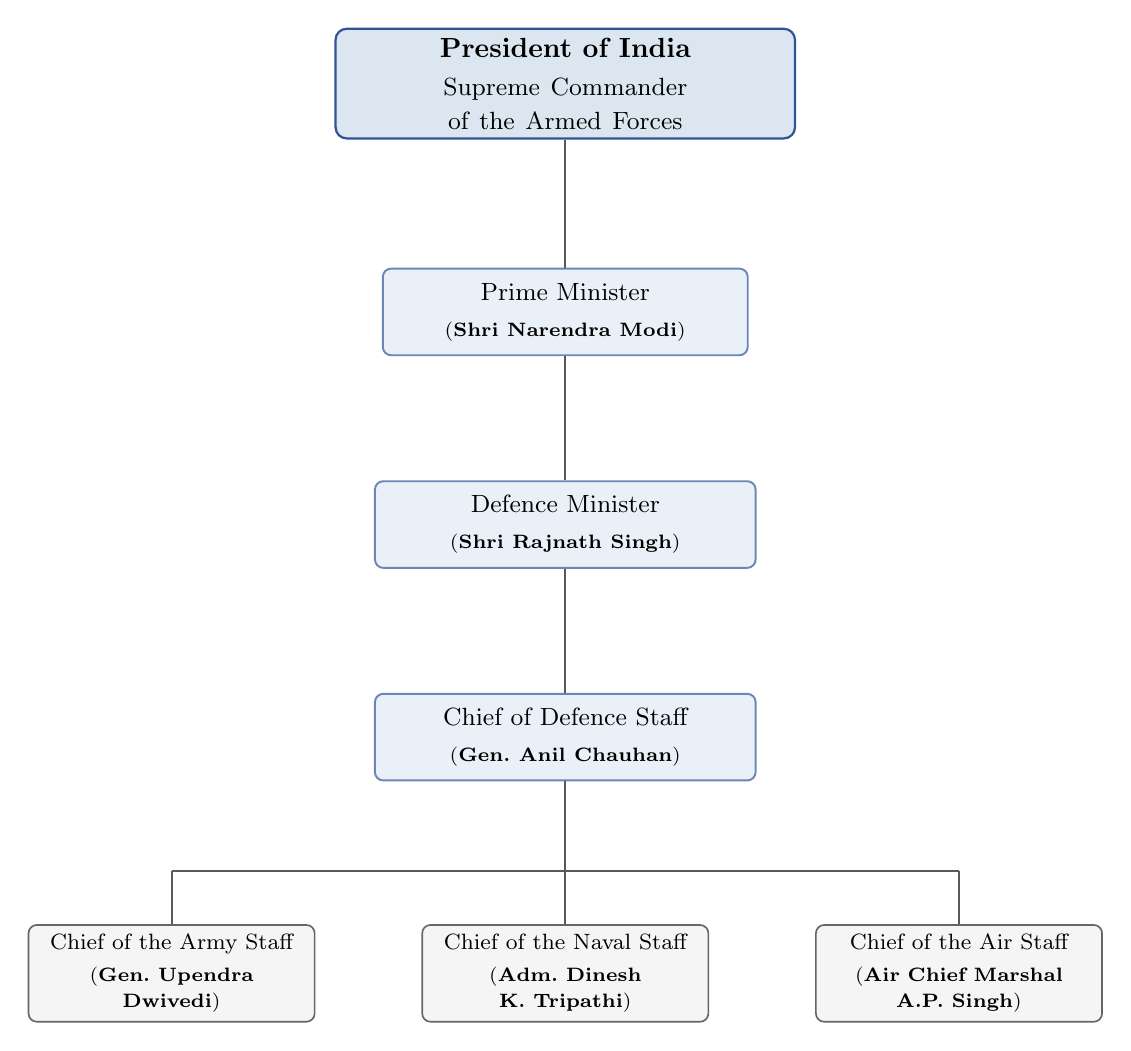
\begin{tikzpicture}
  \node[hroot, text width=5.6cm] (pres) at (0,0)
    {President of India\\[2pt]{\normalfont\small Supreme Commander of the Armed Forces}};

  \node[hlvl, text width=4.4cm] (pm) at (0,-2.9)
    {Prime Minister\\[2pt]{\normalfont\scriptsize (\textbf{Shri Narendra Modi})}};

  \node[hlvl, text width=4.6cm] (dm) at (0,-5.6)
    {Defence Minister\\[2pt]{\normalfont\scriptsize (\textbf{Shri Rajnath Singh})}};

  \node[hlvl, text width=4.6cm] (cds) at (0,-8.3)
    {Chief of Defence Staff\\[2pt]{\normalfont\scriptsize (\textbf{Gen.\ Anil Chauhan})}};

  \node[hleaf, text width=3.4cm] (army) at (-5.0,-11.3)
    {Chief of the Army Staff\\[2pt]{\scriptsize (\textbf{Gen.\ Upendra Dwivedi})}};
  \node[hleaf, text width=3.4cm] (navy) at (0,-11.3)
    {Chief of the Naval Staff\\[2pt]{\scriptsize (\textbf{Adm.\ Dinesh K.\ Tripathi})}};
  \node[hleaf, text width=3.4cm] (af) at (5.0,-11.3)
    {Chief of the Air Staff\\[2pt]{\scriptsize (\textbf{Air Chief Marshal A.P.\ Singh})}};

  \draw[hlink] (pres.south) -- (pm.north);
  \draw[hlink] (pm.south) -- (dm.north);
  \draw[hlink] (dm.south) -- (cds.north);
  \draw[hlink] (cds.south) -- (0,-10.0);
  \draw[hlink] (-5.0,-10.0) -- (5.0,-10.0);
  \draw[hlink] (-5.0,-10.0) -- (army.north);
  \draw[hlink] (0,-10.0) -- (navy.north);
  \draw[hlink] (5.0,-10.0) -- (af.north);
\end{tikzpicture}
\end{center}

\vspace{4pt}
\noindent{\footnotesize
\renewcommand{\arraystretch}{1.18}%
\begin{tabularx}{\textwidth}{@{}>{\raggedright\arraybackslash}p{4.8cm} >{\raggedright\arraybackslash}p{5.2cm} X@{}}
\toprule
\textbf{Office} & \textbf{Holder (October 2026)} & \textbf{Role} \\
\midrule
Defence Minister & \textbf{Shri Rajnath Singh} & Political head of the Ministry of Defence; answers to Parliament for the Armed Forces. \\
\addlinespace[2pt]
Minister of State for Defence & \textbf{Shri Sanjay Seth} & Assists the Defence Minister; Member of Parliament from Ranchi. \\
\addlinespace[2pt]
Defence Secretary & \textbf{Shri Rajesh Kumar Singh} & Administrative head of the Ministry; the Defence Secretary is a civilian officer. \\
\addlinespace[2pt]
Chief of Defence Staff & \textbf{Gen.\ Anil Chauhan} & Principal military adviser to the Government; heads the Department of Military Affairs. \\
\addlinespace[2pt]
Chief of the Army Staff & \textbf{Gen.\ Upendra Dwivedi} & Commands the Indian Army. \\
\addlinespace[2pt]
Chief of the Naval Staff & \textbf{Adm.\ Dinesh K.\ Tripathi} & Commands the Indian Navy. \\
\addlinespace[2pt]
Chief of the Air Staff & \textbf{Air Chief Marshal A.P.\ Singh} & Commands the Indian Air Force. \\
\bottomrule
\end{tabularx}}

\vspace{3pt}
\noindent{\footnotesize\textbf{The chain.} The President is the Supreme Commander; the Defence Minister is politically answerable to Parliament; the CDS coordinates the three services; each Chief commands his service. The Defence Secretary and the service chiefs together form the higher defence organisation.}

% ======================================================= union and states
\newpage
\section*{The Union and the States: How the Centre Reaches Jharkhand}

\noindent{\footnotesize
\renewcommand{\arraystretch}{1.2}%
\begin{tabularx}{\textwidth}{@{}>{\raggedright\arraybackslash}p{4.2cm} >{\raggedright\arraybackslash}p{3.2cm} >{\raggedright\arraybackslash}X@{}}
\toprule
\textbf{Instrument} & \textbf{Provision} & \textbf{Operation in Jharkhand (October 2026)} \\
\midrule
Appointment of the Governor & Art.\ 155 & The President appoints \textbf{Shri Santosh Kumar Gangwar} as Governor of Jharkhand; he holds office during the President's pleasure. \\
\addlinespace[2pt]
Appointment of the Chief Minister & Art.\ 164 & The Governor appoints \textbf{Shri Hemant Soren} as Chief Minister; the other ministers are appointed on the CM's advice. \\
\addlinespace[2pt]
President's Rule & Art.\ 356 & On the Governor's report, the President may assume the functions of the State Government; the Assembly may be suspended or dissolved. \\
\addlinespace[2pt]
All India Services & Art.\ 312 & IAS, IPS and IFoS officers of the Jharkhand cadre serve both the Union and the State; the Chief Secretary is \textbf{Shri Avinash Kumar}. \\
\addlinespace[2pt]
Finance Commission & Art.\ 280 & The 16th Finance Commission, chaired by \textbf{Dr.\ Arvind Panagariya}, recommends Jharkhand's share of central taxes and grants-in-aid. \\
\addlinespace[2pt]
Inter-State Council & Art.\ 263 & A forum for consultation between the Union and the States on matters of common interest. \\
\addlinespace[2pt]
NITI Aayog & Executive & Policy support and monitoring, including the Aspirational Districts Programme in which Jharkhand districts participate. \\
\addlinespace[2pt]
Centrally sponsored schemes & Legislation and executive instructions & Implemented through State departments and district offices; funds flow from the Union Ministry to the State and then to the district. \\
\bottomrule
\end{tabularx}}

\vspace{4pt}
\noindent{\footnotesize\textbf{Key office holders in Jharkhand.}}

\vspace{2pt}
\noindent{\footnotesize
\renewcommand{\arraystretch}{1.16}%
\begin{tabularx}{\textwidth}{@{}>{\raggedright\arraybackslash}p{7.0cm} >{\raggedright\arraybackslash}p{8.4cm}@{}}
\toprule
\textbf{Office} & \textbf{Holder (October 2026)} \\
\midrule
Governor of Jharkhand & \textbf{Shri Santosh Kumar Gangwar} \\
\addlinespace[2pt]
Chief Minister of Jharkhand & \textbf{Shri Hemant Soren} \\
\addlinespace[2pt]
Chief Secretary, Jharkhand & \textbf{Shri Avinash Kumar} \\
\addlinespace[2pt]
Director General of Police, Jharkhand & \textbf{Smt.\ Tadasha Mishra} \\
\addlinespace[2pt]
Chief Justice, Jharkhand High Court & \textbf{Justice Mahesh Sharadchandra Sonak} \\
\addlinespace[2pt]
Advocate General, Jharkhand & \textbf{Shri Rohitashya Roy} \\
\addlinespace[2pt]
Deputy Commissioner, Ranchi & \textbf{Shri Manjunath Bhajantri, IAS} \\
\addlinespace[2pt]
Senior Superintendent of Police, Ranchi & \textbf{Shri Rakesh Ranjan} \\
\bottomrule
\end{tabularx}}

% ======================================================= worked example admin
\newpage
\section*{A Worked Example: From the Union to Muri}

\begin{center}
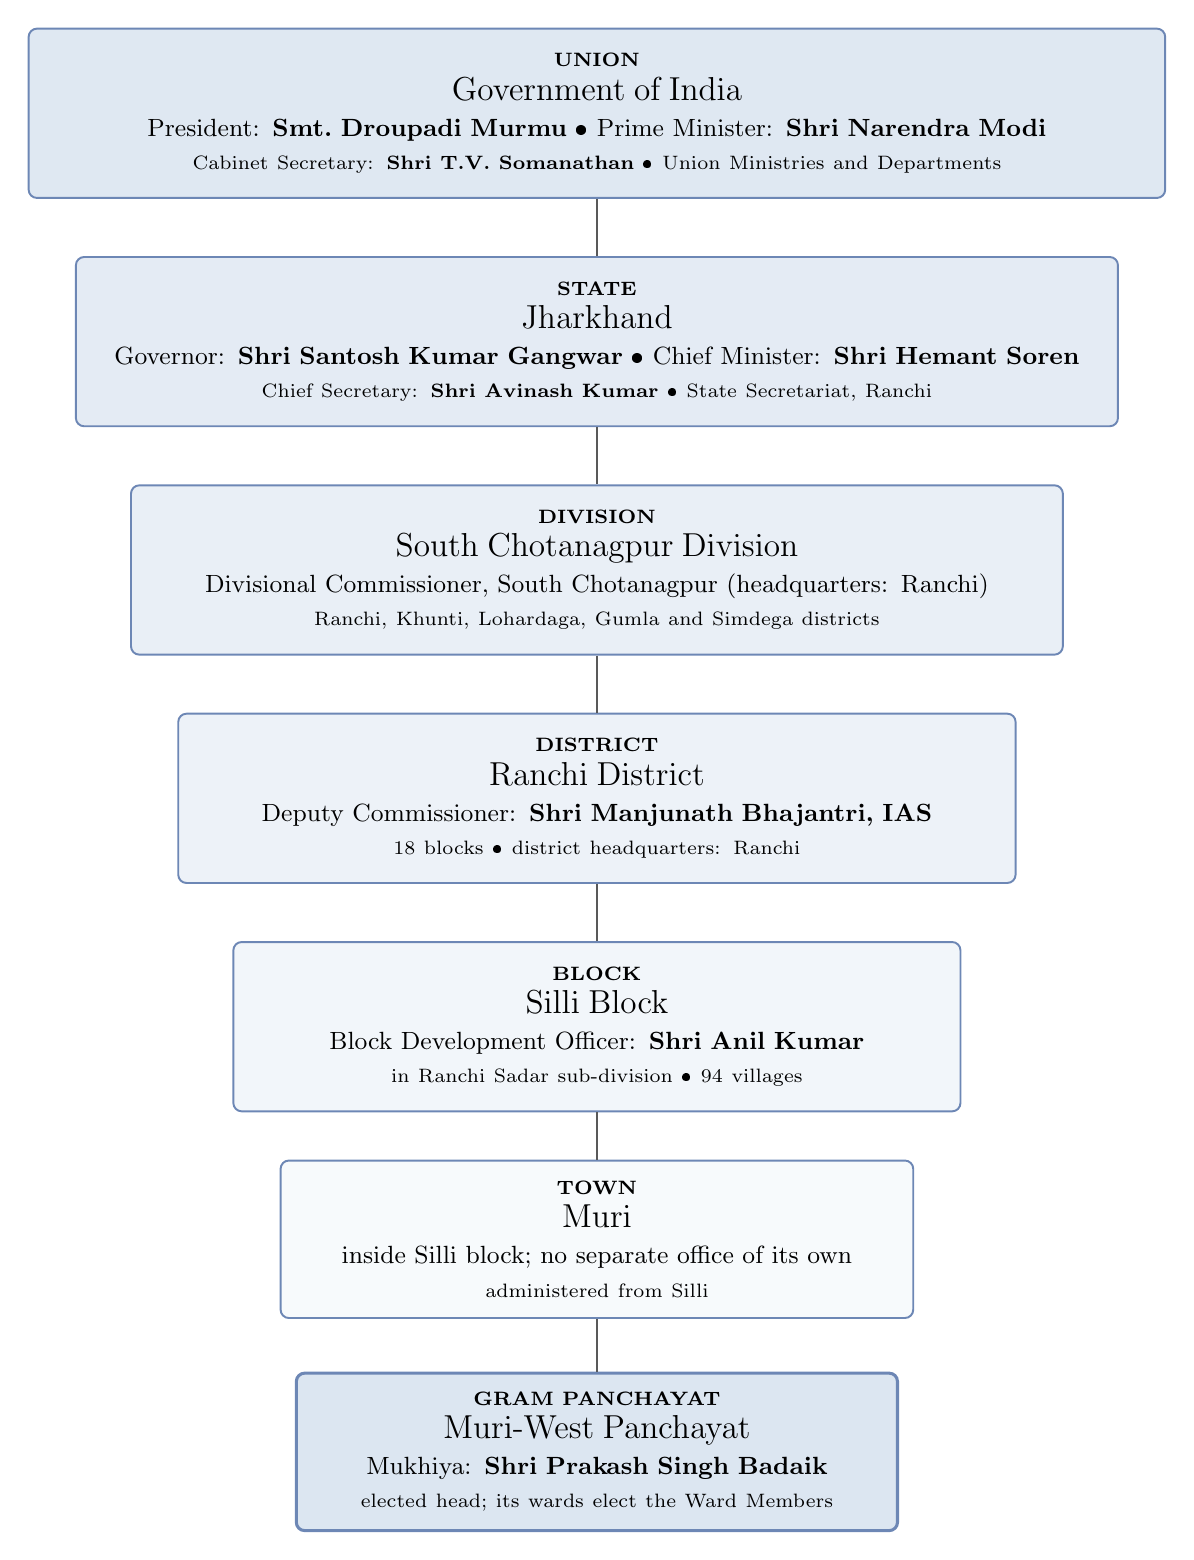
\begin{tikzpicture}
  \node[elecbox, text width=14.2cm, minimum height=2.15cm, fill=apexfill!90] (union) at (0,0)
    {{\scriptsize\textbf{UNION}}\\[1pt]
     {\large Government of India}\\[2pt]
     {President: \textbf{Smt.\ Droupadi Murmu} \textbullet\ Prime Minister: \textbf{Shri Narendra Modi}}\\[1pt]
     {\scriptsize Cabinet Secretary: \textbf{Shri T.V.\ Somanathan} \textbullet\ Union Ministries and Departments}};

  \node[elecbox, text width=13.0cm, minimum height=2.15cm, fill=apexfill!78] (state) at (0,-2.9)
    {{\scriptsize\textbf{STATE}}\\[1pt]
     {\large Jharkhand}\\[2pt]
     {Governor: \textbf{Shri Santosh Kumar Gangwar} \textbullet\ Chief Minister: \textbf{Shri Hemant Soren}}\\[1pt]
     {\scriptsize Chief Secretary: \textbf{Shri Avinash Kumar} \textbullet\ State Secretariat, Ranchi}};

  \node[elecbox, text width=11.6cm, minimum height=2.15cm, fill=apexfill!64] (div) at (0,-5.8)
    {{\scriptsize\textbf{DIVISION}}\\[1pt]
     {\large South Chotanagpur Division}\\[2pt]
     {Divisional Commissioner, South Chotanagpur (headquarters: Ranchi)}\\[1pt]
     {\scriptsize Ranchi, Khunti, Lohardaga, Gumla and Simdega districts}};

  \node[elecbox, text width=10.4cm, minimum height=2.15cm, fill=apexfill!50] (dist) at (0,-8.7)
    {{\scriptsize\textbf{DISTRICT}}\\[1pt]
     {\large Ranchi District}\\[2pt]
     {Deputy Commissioner: \textbf{Shri Manjunath Bhajantri, IAS}}\\[1pt]
     {\scriptsize 18 blocks \textbullet\ district headquarters: Ranchi}};

  \node[elecbox, text width=9.0cm, minimum height=2.15cm, fill=apexfill!36] (blk) at (0,-11.6)
    {{\scriptsize\textbf{BLOCK}}\\[1pt]
     {\large Silli Block}\\[2pt]
     {Block Development Officer: \textbf{Shri Anil Kumar}}\\[1pt]
     {\scriptsize in Ranchi Sadar sub-division \textbullet\ 94 villages}};

  \node[elecbox, text width=7.8cm, minimum height=2.0cm, fill=apexfill!22] (town) at (0,-14.3)
    {{\scriptsize\textbf{TOWN}}\\[1pt]
     {\large Muri}\\[2pt]
     {inside Silli block; no separate office of its own}\\[1pt]
     {\scriptsize administered from Silli}};

  \node[elecbox, text width=7.4cm, minimum height=2.0cm, fill=apexfill, line width=1.1pt] (gp) at (0,-17.0)
    {{\scriptsize\textbf{GRAM PANCHAYAT}}\\[1pt]
     {\large Muri-West Panchayat}\\[2pt]
     {Mukhiya: \textbf{Shri Prakash Singh Badaik}}\\[1pt]
     {\scriptsize elected head; its wards elect the Ward Members}};

  \draw[hlink] (union.south) -- (state.north);
  \draw[hlink] (state.south) -- (div.north);
  \draw[hlink] (div.south) -- (dist.north);
  \draw[hlink] (dist.south) -- (blk.north);
  \draw[hlink] (blk.south) -- (town.north);
  \draw[hlink] (town.south) -- (gp.north);
\end{tikzpicture}
\end{center}

\vspace{2pt}
\noindent{\footnotesize\textbf{Reading the example.} The Union makes policy and funds, the State adapts and implements it, the division coordinates districts, and the district, block and panchayat carry it to the village. Silli is a block, not a sub-division, and Muri is a town inside Silli block --- so the chain runs State $\rightarrow$ Division $\rightarrow$ District $\rightarrow$ Block $\rightarrow$ Gram Panchayat, with Muri marking the locality, not a separate tier. Names are as of 2026; the BDO and Mukhiya follow the latest district records (2024--25).}

% ======================================================= police chain
\newpage
\section*{A Worked Example: The Police Chain from the Union to Muri Thana}

\begin{center}
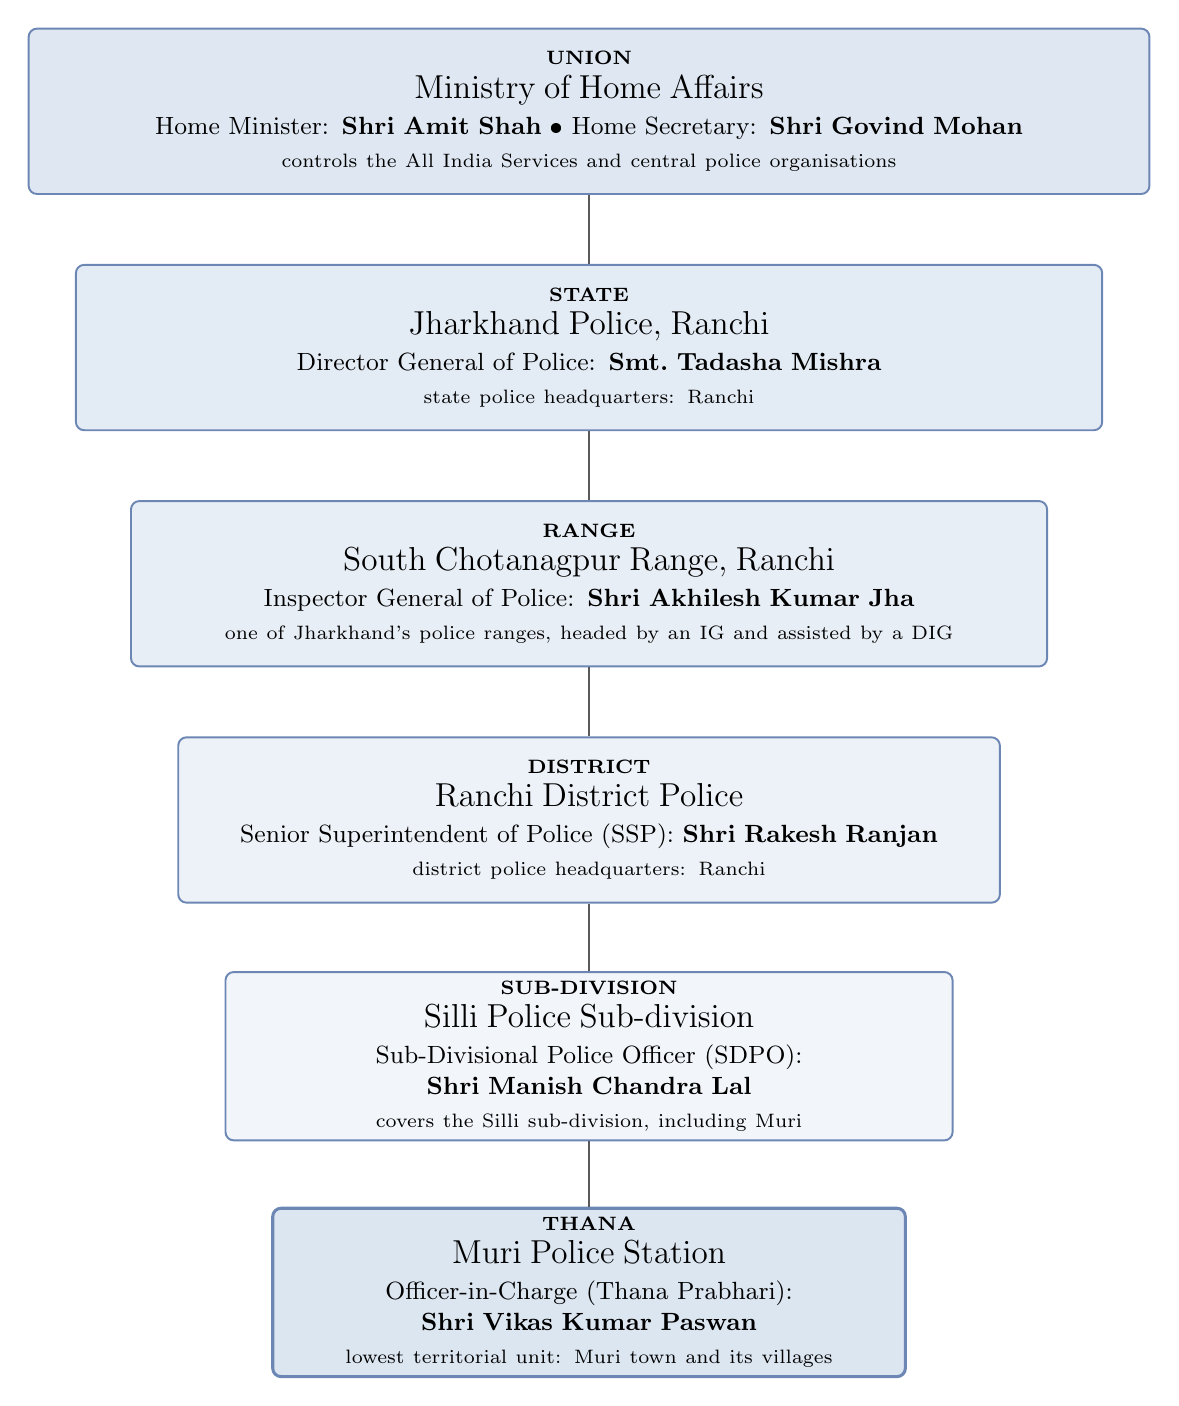
\begin{tikzpicture}
  \node[elecbox, text width=14.0cm, minimum height=2.1cm, fill=apexfill!92] (mha) at (0,0)
    {{\scriptsize\textbf{UNION}}\\[1pt]
     {\large Ministry of Home Affairs}\\[2pt]
     {Home Minister: \textbf{Shri Amit Shah} \textbullet\ Home Secretary: \textbf{Shri Govind Mohan}}\\[1pt]
     {\scriptsize controls the All India Services and central police organisations}};

  \node[elecbox, text width=12.8cm, minimum height=2.1cm, fill=apexfill!80] (dgp) at (0,-3.0)
    {{\scriptsize\textbf{STATE}}\\[1pt]
     {\large Jharkhand Police, Ranchi}\\[2pt]
     {Director General of Police: \textbf{Smt.\ Tadasha Mishra}}\\[1pt]
     {\scriptsize state police headquarters: Ranchi}};

  \node[elecbox, text width=11.4cm, minimum height=2.1cm, fill=apexfill!66] (range) at (0,-6.0)
    {{\scriptsize\textbf{RANGE}}\\[1pt]
     {\large South Chotanagpur Range, Ranchi}\\[2pt]
     {Inspector General of Police: \textbf{Shri Akhilesh Kumar Jha}}\\[1pt]
     {\scriptsize one of Jharkhand's police ranges, headed by an IG and assisted by a DIG}};

  \node[elecbox, text width=10.2cm, minimum height=2.1cm, fill=apexfill!52] (ssp) at (0,-9.0)
    {{\scriptsize\textbf{DISTRICT}}\\[1pt]
     {\large Ranchi District Police}\\[2pt]
     {Senior Superintendent of Police (SSP): \textbf{Shri Rakesh Ranjan}}\\[1pt]
     {\scriptsize district police headquarters: Ranchi}};

  \node[elecbox, text width=9.0cm, minimum height=2.1cm, fill=apexfill!38] (sdpo) at (0,-12.0)
    {{\scriptsize\textbf{SUB-DIVISION}}\\[1pt]
     {\large Silli Police Sub-division}\\[2pt]
     {Sub-Divisional Police Officer (SDPO): \textbf{Shri Manish Chandra Lal}}\\[1pt]
     {\scriptsize covers the Silli sub-division, including Muri}};

  \node[elecbox, text width=7.8cm, minimum height=2.1cm, fill=apexfill, line width=1.1pt] (thana) at (0,-15.0)
    {{\scriptsize\textbf{THANA}}\\[1pt]
     {\large Muri Police Station}\\[2pt]
     {Officer-in-Charge (Thana Prabhari): \textbf{Shri Vikas Kumar Paswan}}\\[1pt]
     {\scriptsize lowest territorial unit: Muri town and its villages}};

  \draw[hlink] (mha.south) -- (dgp.north);
  \draw[hlink] (dgp.south) -- (range.north);
  \draw[hlink] (range.south) -- (ssp.north);
  \draw[hlink] (ssp.south) -- (sdpo.north);
  \draw[hlink] (sdpo.south) -- (thana.north);
\end{tikzpicture}
\end{center}

\vspace{2pt}
\noindent{\footnotesize\textbf{Reading the example.} The Union Home Ministry controls the All India Services and lays down national policing policy; the State DGP commands the State police; the range IG supervises the districts in the range; the SSP commands the district; the SDPO a police sub-division; and the thana in-charge the police station --- the lowest territorial unit of policing. Names are as of 2026; the SDPO and the thana in-charge took their posts in the May 2026 reshuffle.}

% ======================================================= election hierarchy
\newpage
\section*{Election Hierarchy: From the President to the Ward Member}

\noindent{\footnotesize Elections to the offices below are conducted by the Election Commission of India, headed by Chief Election Commissioner \textbf{Shri Gyanesh Kumar}. The diagram separates national elections (left) from State and local elections (right).}

\vspace{6pt}
\begin{center}
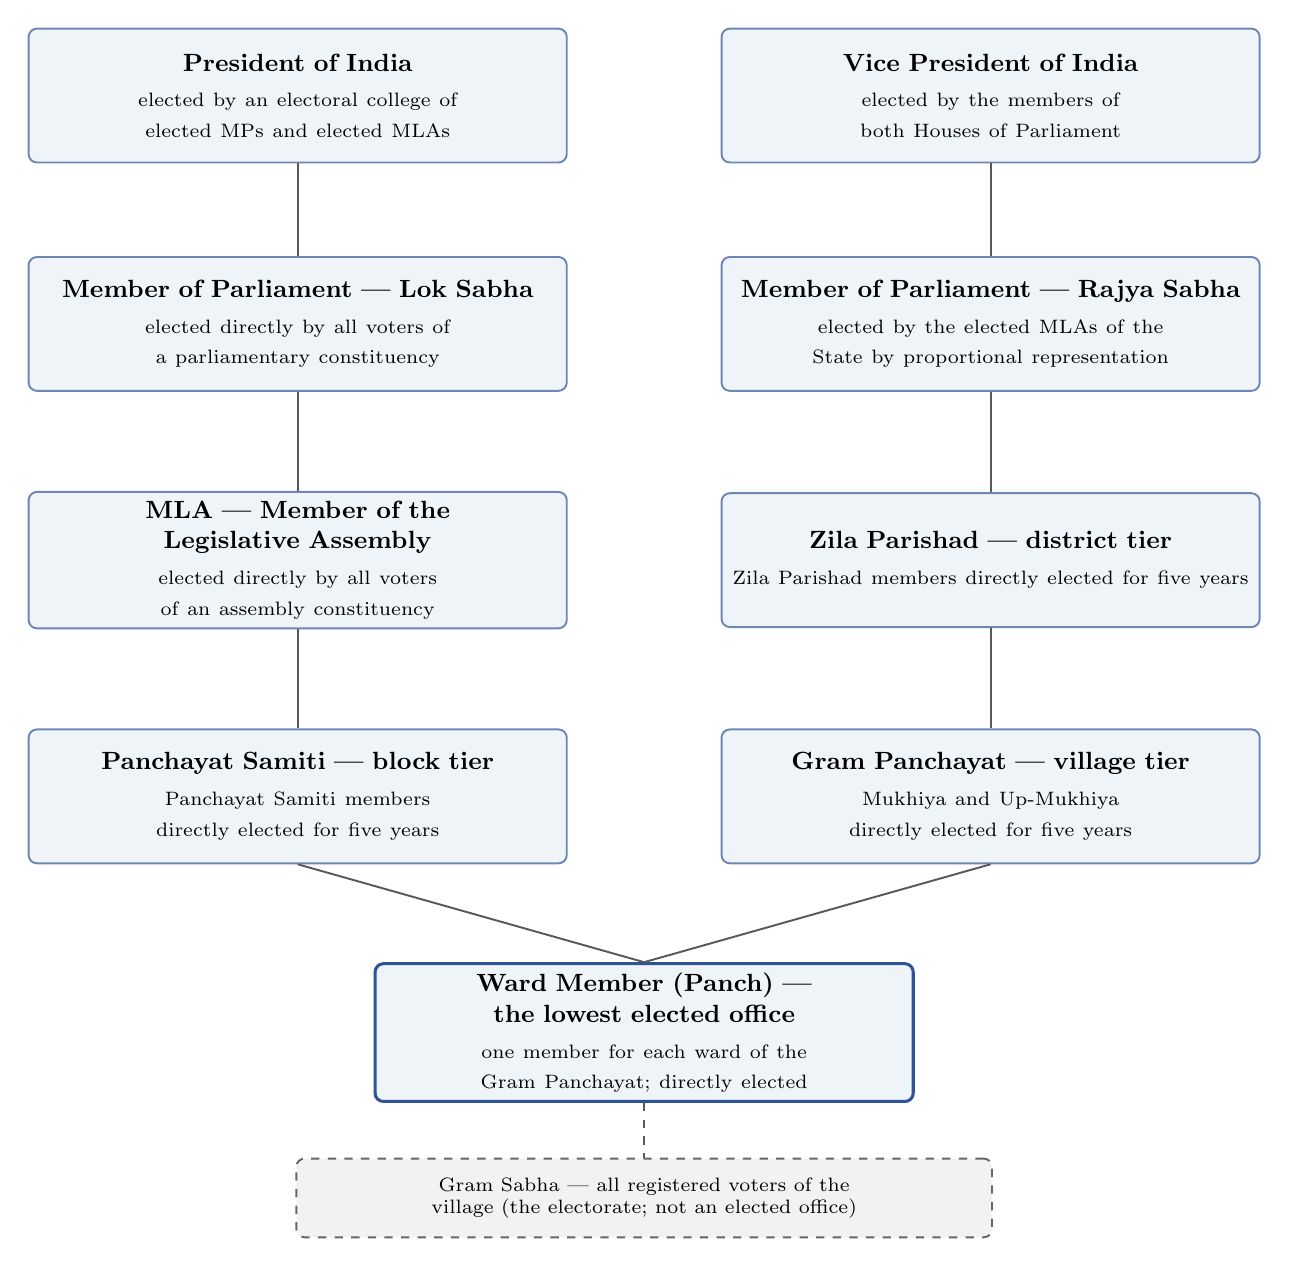
\begin{tikzpicture}
  \node[elecbox, text width=6.6cm, minimum height=1.7cm] (pres) at (-4.4,0)
    {\textbf{President of India}\\[2pt]
     {\scriptsize elected by an electoral college of elected MPs and elected MLAs}};
  \node[elecbox, text width=6.6cm, minimum height=1.7cm] (vp) at (4.4,0)
    {\textbf{Vice President of India}\\[2pt]
     {\scriptsize elected by the members of both Houses of Parliament}};

  \node[elecbox, text width=6.6cm, minimum height=1.7cm] (ls) at (-4.4,-2.9)
    {\textbf{Member of Parliament --- Lok Sabha}\\[2pt]
     {\scriptsize elected directly by all voters of a parliamentary constituency}};
  \node[elecbox, text width=6.6cm, minimum height=1.7cm] (rs) at (4.4,-2.9)
    {\textbf{Member of Parliament --- Rajya Sabha}\\[2pt]
     {\scriptsize elected by the elected MLAs of the State by proportional representation}};

  \node[elecbox, text width=6.6cm, minimum height=1.7cm] (mla) at (-4.4,-5.9)
    {\textbf{MLA --- Member of the Legislative Assembly}\\[2pt]
     {\scriptsize elected directly by all voters of an assembly constituency}};
  \node[elecbox, text width=6.6cm, minimum height=1.7cm] (zp) at (4.4,-5.9)
    {\textbf{Zila Parishad --- district tier}\\[2pt]
     {\scriptsize Zila Parishad members directly elected for five years}};

  \node[elecbox, text width=6.6cm, minimum height=1.7cm] (ps) at (-4.4,-8.9)
    {\textbf{Panchayat Samiti --- block tier}\\[2pt]
     {\scriptsize Panchayat Samiti members directly elected for five years}};
  \node[elecbox, text width=6.6cm, minimum height=1.7cm] (gp) at (4.4,-8.9)
    {\textbf{Gram Panchayat --- village tier}\\[2pt]
     {\scriptsize Mukhiya and Up-Mukhiya directly elected for five years}};

  \node[elecbox, text width=6.6cm, minimum height=1.7cm, draw=apexline, line width=1.1pt] (ward) at (0,-11.9)
    {\textbf{Ward Member (Panch) --- the lowest elected office}\\[2pt]
     {\scriptsize one member for each ward of the Gram Panchayat; directly elected}};

  \node[elecbox, draw=subline, dashed, fill=subfill, font=\scriptsize,
        minimum height=1.0cm, text width=8.6cm] (gs) at (0,-14.0)
    {Gram Sabha --- all registered voters of the village (the electorate; not an elected office)};

  \draw[hlink] (pres.south) -- (ls.north);
  \draw[hlink] (ls.south) -- (mla.north);
  \draw[hlink] (vp.south) -- (rs.north);
  \draw[hlink] (rs.south) -- (zp.north);
  \draw[hlink] (zp.south) -- (gp.north);
  \draw[hlink] (mla.south) -- (ps.north);
  \draw[hlink] (ps.south) -- (ward.north);
  \draw[hlink] (gp.south) -- (ward.north);
  \draw[hlink, dashed] (ward.south) -- (gs.north);
\end{tikzpicture}
\end{center}

\vspace{2pt}
\noindent{\footnotesize\textbf{How to read this.} The left column is the national and State legislative chain; the right column is the local-government chain. The vertical order shows the level of government --- Union, State, district, block, village, ward --- not a chain of command. Above the MLA sits the MP; in towns the parallel of the panchayat tiers is the Municipal Corporation, whose wards elect Councillors. The President and the Vice President are elected indirectly; all other offices shown are filled by direct election.}

% ======================================================= Jharkhand representation
\newpage
\section*{Jharkhand's Representation in the Union}

\noindent{\footnotesize Jharkhand sends 14 members to the Lok Sabha and 6 to the Rajya Sabha; its 81 MLAs form the electoral college for the State's Rajya Sabha seats. The State's Members of Parliament are listed below.}

\vspace{4pt}
\noindent{\footnotesize
\renewcommand{\arraystretch}{1.16}%
\begin{longtable}{@{}>{\raggedright\arraybackslash}p{4.0cm} >{\raggedright\arraybackslash}p{7.4cm} >{\raggedright\arraybackslash}p{3.2cm}@{}}
\toprule
\textbf{Lok Sabha constituency} & \textbf{Member of Parliament} & \textbf{Party} \\
\midrule
\endfirsthead
\toprule
\textbf{Lok Sabha constituency} & \textbf{Member of Parliament} & \textbf{Party} \\
\midrule
\endhead
Rajmahal & \textbf{Shri Vijay Hansda} & JMM \\
\addlinespace[2pt]
Dumka & \textbf{Shri Nalin Soren} & JMM \\
\addlinespace[2pt]
Godda & \textbf{Shri Nishikant Dubey} & BJP \\
\addlinespace[2pt]
Chatra & \textbf{Shri Kalicharan Singh} & BJP \\
\addlinespace[2pt]
Kodarma & \textbf{Smt.\ Annapurna Devi} & BJP \\
\addlinespace[2pt]
Giridih & \textbf{Shri Chandra Prakash Choudhary} & AJSU \\
\addlinespace[2pt]
Dhanbad & \textbf{Shri Dulu Mahato} & BJP \\
\addlinespace[2pt]
Ranchi & \textbf{Shri Sanjay Seth} & BJP \\
\addlinespace[2pt]
Jamshedpur & \textbf{Shri Bidyut Baran Mahato} & BJP \\
\addlinespace[2pt]
Singhbhum & \textbf{Smt.\ Joba Majhi} & JMM \\
\addlinespace[2pt]
Khunti & \textbf{Shri Kali Charan Munda} & BJP \\
\addlinespace[2pt]
Lohardaga & \textbf{Shri Sukhdeo Bhagat} & Congress \\
\addlinespace[2pt]
Palamu & \textbf{Shri Vishnu Dayal Ram} & BJP \\
\addlinespace[2pt]
Hazaribagh & \textbf{Shri Manish Jaiswal} & BJP \\
\bottomrule
\end{longtable}}

\vspace{4pt}
\noindent{\footnotesize\textbf{Union Ministers from Jharkhand.} \textbf{Smt.\ Annapurna Devi} (Kodarma) is Cabinet Minister for Women and Child Development; \textbf{Shri Sanjay Seth} (Ranchi) is Minister of State for Defence. Both sit in the Union Council of Ministers listed earlier.}

\vspace{6pt}
\noindent{\footnotesize
\renewcommand{\arraystretch}{1.18}%
\begin{tabularx}{\textwidth}{@{}>{\raggedright\arraybackslash}p{6.8cm} >{\raggedright\arraybackslash}p{8.5cm}@{}}
\toprule
\textbf{Jharkhand in the Union} & \textbf{Number / note} \\
\midrule
Lok Sabha seats & 14 \\
\addlinespace[2pt]
Rajya Sabha seats & 6 (elected by the 81 MLAs) \\
\addlinespace[2pt]
Legislative Assembly seats & 81 \\
\addlinespace[2pt]
Administrative divisions & 5 --- North Chotanagpur, South Chotanagpur, Palamu, Kolhan, Santhal Pargana \\
\addlinespace[2pt]
Districts & 24 \\
\addlinespace[2pt]
Blocks & 264 \\
\addlinespace[2pt]
Gram Panchayats & about 4,345 \\
\bottomrule
\end{tabularx}}

\vspace{3pt}
\noindent{\scriptsize The Rajya Sabha members elected in 2022 and 2024 --- \textbf{Smt.\ Mahua Maji}, \textbf{Shri Aditya Sahu}, \textbf{Shri Sarfaraz Ahmad} and \textbf{Shri Pradeep Verma} --- continue in the House; the two seats that fell due in 2026 were filled at the biennial election.}

% ======================================================= national programmes
\newpage
\section*{National Programmes at Muri}

\noindent{\footnotesize The following Union programmes reach Muri through the State Government, the district administration and the block. The nodal Ministry and the responsible Union Minister are shown against each.}

\vspace{4pt}
\noindent{\footnotesize
\renewcommand{\arraystretch}{1.18}%
\begin{longtable}{@{}>{\raggedright\arraybackslash}p{3.7cm} >{\raggedright\arraybackslash}p{3.0cm} >{\raggedright\arraybackslash}p{4.1cm} >{\raggedright\arraybackslash}p{3.8cm}@{}}
\toprule
\textbf{Programme} & \textbf{Nodal Ministry} & \textbf{Union Minister} & \textbf{What it does at Muri} \\
\midrule
\endfirsthead
\toprule
\textbf{Programme} & \textbf{Nodal Ministry} & \textbf{Union Minister} & \textbf{What it does at Muri} \\
\midrule
\endhead
\textbf{MGNREGA} & Rural Development & \textbf{Shri Shivraj Singh Chouhan} & Wage employment on rural works; implemented through the Silli block. \\
\addlinespace[2pt]
\textbf{PMAY--Gramin} & Rural Development & \textbf{Shri Shivraj Singh Chouhan} & Assistance for pucca houses for eligible rural families. \\
\addlinespace[2pt]
\textbf{PMGSY} & Rural Development & \textbf{Shri Shivraj Singh Chouhan} & All-weather rural roads linking villages around Muri. \\
\addlinespace[2pt]
\textbf{Jal Jeevan Mission} & Jal Shakti & \textbf{Shri C.R.\ Patil} & Piped drinking water to rural households. \\
\addlinespace[2pt]
\textbf{Swachh Bharat Mission (Gramin)} & Jal Shakti & \textbf{Shri C.R.\ Patil} & Sanitation and solid and liquid waste management in villages. \\
\addlinespace[2pt]
\textbf{Ayushman Bharat (PM-JAY)} & Health and Family Welfare & \textbf{Shri J.P.\ Nadda} & Health cover for eligible families; treatment at empanelled hospitals. \\
\addlinespace[2pt]
\textbf{PM-KISAN} & Agriculture and Farmers Welfare & \textbf{Shri Shivraj Singh Chouhan} & Income support to eligible landholding farmers. \\
\addlinespace[2pt]
\textbf{National Food Security Act} & Consumer Affairs, Food and Public Distribution & \textbf{Shri Pralhad Joshi} & Subsidised foodgrain through the public distribution system. \\
\addlinespace[2pt]
\textbf{Pradhan Mantri Ujjwala Yojana} & Petroleum and Natural Gas & \textbf{Shri Hardeep Singh Puri} & LPG connections for women from eligible households. \\
\addlinespace[2pt]
\textbf{Saubhagya} & Power & \textbf{Shri Manohar Lal Khattar} & Household electrification in unconnected rural areas. \\
\addlinespace[2pt]
\textbf{PM Vishwakarma} & Micro, Small and Medium Enterprises & \textbf{Shri Jitan Ram Manjhi} & Support to traditional artisans and craftspeople. \\
\addlinespace[2pt]
\textbf{Skill India Mission} & Skill Development and Entrepreneurship & \textbf{Shri Jayant Chaudhary} & Short-term skill training and certification through the block. \\
\addlinespace[2pt]
\textbf{Aspirational Districts Programme} & NITI Aayog & \textbf{Shri Narendra Modi} (Chairperson) & District-level monitoring of health, education, agriculture and basic infrastructure. \\
\bottomrule
\end{longtable}}

\vspace{3pt}
\noindent{\scriptsize Ministries and Ministers as of October 2026; scheme implementation at the district level is carried out by the Deputy Commissioner and the Block Development Officer, with the Panchayat as the last-mile institution.}

% ======================================================= Muri sector page
\newpage
\section*{Muri at a Glance: How the National System Touches the Town}

\begin{center}
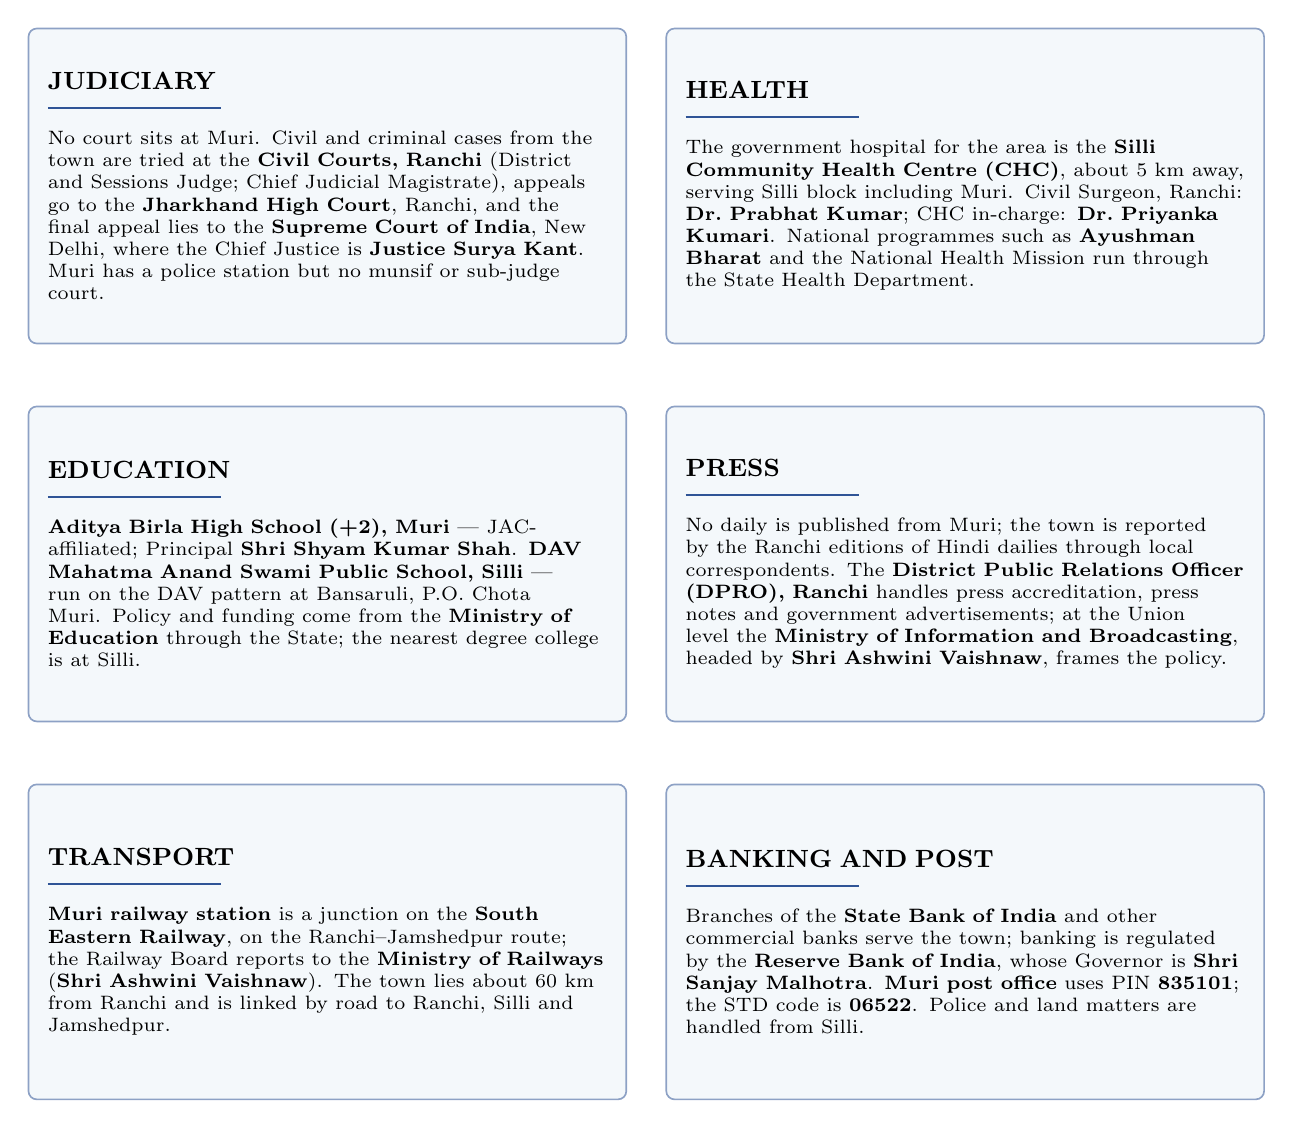
\begin{tikzpicture}
  \node[secbox] at (-4.05,-0.2)
    {{\textbf{\small JUDICIARY}}\\[-1pt]{\color{apexline}\rule{2.2cm}{0.7pt}}\\[5pt]
     No court sits at Muri. Civil and criminal cases from the town are tried at the
     \textbf{Civil Courts, Ranchi} (District and Sessions Judge; Chief Judicial Magistrate),
     appeals go to the \textbf{Jharkhand High Court}, Ranchi, and the final appeal lies to the
     \textbf{Supreme Court of India}, New Delhi, where the Chief Justice is
     \textbf{Justice Surya Kant}. Muri has a police station but no munsif or sub-judge court.};

  \node[secbox] at (4.05,-0.2)
    {{\textbf{\small HEALTH}}\\[-1pt]{\color{apexline}\rule{2.2cm}{0.7pt}}\\[5pt]
     The government hospital for the area is the \textbf{Silli Community Health Centre (CHC)},
     about 5 km away, serving Silli block including Muri. Civil Surgeon, Ranchi:
     \textbf{Dr.\ Prabhat Kumar}; CHC in-charge: \textbf{Dr.\ Priyanka Kumari}. National
     programmes such as \textbf{Ayushman Bharat} and the National Health Mission run through
     the State Health Department.};

  \node[secbox] at (-4.05,-5.0)
    {{\textbf{\small EDUCATION}}\\[-1pt]{\color{apexline}\rule{2.2cm}{0.7pt}}\\[5pt]
     \textbf{Aditya Birla High School (+2), Muri} --- JAC-affiliated; Principal
     \textbf{Shri Shyam Kumar Shah}. \textbf{DAV Mahatma Anand Swami Public School, Silli}
     --- run on the DAV pattern at Bansaruli, P.O.\ Chota Muri. Policy and funding come from
     the \textbf{Ministry of Education} through the State; the nearest degree college is at Silli.};

  \node[secbox] at (4.05,-5.0)
    {{\textbf{\small PRESS}}\\[-1pt]{\color{apexline}\rule{2.2cm}{0.7pt}}\\[5pt]
     No daily is published from Muri; the town is reported by the Ranchi editions of Hindi
     dailies through local correspondents. The \textbf{District Public Relations Officer
     (DPRO), Ranchi} handles press accreditation, press notes and government advertisements;
     at the Union level the \textbf{Ministry of Information and Broadcasting}, headed by
     \textbf{Shri Ashwini Vaishnaw}, frames the policy.};

  \node[secbox] at (-4.05,-9.8)
    {{\textbf{\small TRANSPORT}}\\[-1pt]{\color{apexline}\rule{2.2cm}{0.7pt}}\\[5pt]
     \textbf{Muri railway station} is a junction on the \textbf{South Eastern Railway}, on the
     Ranchi--Jamshedpur route; the Railway Board reports to the
     \textbf{Ministry of Railways} (\textbf{Shri Ashwini Vaishnaw}). The town lies about 60 km
     from Ranchi and is linked by road to Ranchi, Silli and Jamshedpur.};

  \node[secbox] at (4.05,-9.8)
    {{\textbf{\small BANKING AND POST}}\\[-1pt]{\color{apexline}\rule{2.2cm}{0.7pt}}\\[5pt]
     Branches of the \textbf{State Bank of India} and other commercial banks serve the town;
     banking is regulated by the \textbf{Reserve Bank of India}, whose Governor is
     \textbf{Shri Sanjay Malhotra}. \textbf{Muri post office} uses PIN \textbf{835101}; the
     STD code is \textbf{06522}. Police and land matters are handled from Silli.};
\end{tikzpicture}
\end{center}

\vspace{2pt}
\noindent{\footnotesize Sector details are as per the latest available district records and reports (2024--26); the police set-up is described in the worked example on the earlier page.}

\end{document}
